% !TEX program = pdflatex
% =============================================================================
%  Reporte técnico · Entrega 2 · Graduación UNAL
%  Estructuras de Datos (2016699) · Universidad Nacional de Colombia
%
%  Compilar dos veces (índice y referencias cruzadas):
%      pdflatex Proyecto-Entrega2-Reporte.tex
%  En Overleaf: suba este archivo y la carpeta figuras/ y use pdfLaTeX.
%
%  Lo que falta está marcado con \pendiente{...} y sale en rojo en el PDF:
%  el número del equipo (portada y nombre del PDF: Proyecto-Entrega2-Reporte-<número>.pdf)
%  y el enlace del video (secciones 1 y 11).
%
%  Las tablas y gráficas de tiempos (sección 9) se arman con tiempos_resumen.csv y
%  cuadraticas_resumen.csv, que deben estar junto a este archivo (o en ../resultados/).
%  Para medir de nuevo: tarea de VS Code "Graduación UNAL: mediciones para el reporte".
% =============================================================================

\documentclass[11pt,letterpaper]{article}

% ---------------------------------------------------------------- idioma y fuentes
\usepackage[T1]{fontenc}
\usepackage[utf8]{inputenc}
\usepackage{lmodern}
\usepackage[spanish,es-tabla,es-noshorthands]{babel}
\usepackage{microtype}

% ---------------------------------------------------------------- página
\usepackage[margin=2.5cm,headheight=14pt]{geometry}
\usepackage{fancyhdr}
\usepackage{titlesec}
\usepackage{enumitem}
\setlist{itemsep=2pt,topsep=4pt}
\usepackage{needspace}
\usepackage[titles]{tocloft}
\setlength{\cftsecnumwidth}{2em}
\setlength{\cftsubsecnumwidth}{2.8em}
\renewcommand{\cftsecaftersnum}{.}
\renewcommand{\cftsubsecaftersnum}{.}

% ---------------------------------------------------------------- matemáticas, tablas, figuras
\usepackage{amsmath,amssymb}
\usepackage{graphicx}
\usepackage{xcolor}
\usepackage{booktabs,tabularx,array,multirow}
\newcolumntype{L}{>{\raggedright\arraybackslash}X}
\newcolumntype{P}[1]{>{\raggedright\arraybackslash}p{#1}}
\usepackage{caption}
\captionsetup{font=small,labelfont=bf}
\usepackage{float}
\usepackage{listings}
\usepackage{tikz}
\usetikzlibrary{arrows.meta,positioning,shapes.geometric,calc}
\usepackage{pgfplots}
\usepackage{pgfplotstable}
\pgfplotsset{compat=1.18}
\usepackage[hidelinks]{hyperref}

% ---------------------------------------------------------------- colores
\definecolor{azulun}{HTML}{1F4E79}
\definecolor{rojo}{HTML}{B3261E}
\definecolor{gris}{HTML}{6B6B6B}
\definecolor{naranja}{HTML}{C0581F}
\definecolor{verde}{HTML}{2E7D4F}
\definecolor{morado}{HTML}{6A3D9A}
\definecolor{fondocodigo}{HTML}{F5F6F8}

\hypersetup{
  colorlinks=true, linkcolor=azulun, citecolor=azulun, urlcolor=azulun,
  pdftitle={Graduación UNAL - Reporte técnico, Entrega 2},
  pdfsubject={Estructuras de Datos (2016699), Universidad Nacional de Colombia},
}

\titleformat*{\section}{\Large\bfseries\color{azulun}}
\titleformat*{\subsection}{\large\bfseries\color{azulun}}
\titleformat*{\subsubsection}{\normalsize\bfseries}

\pagestyle{fancy}
\fancyhf{}
\fancyhead[L]{\small\color{gris}Graduación UNAL · Reporte técnico, Entrega 2}
\fancyhead[R]{\small\color{gris}\thepage}
\renewcommand{\headrulewidth}{0.4pt}

% ---------------------------------------------------------------- partes pendientes
\newcommand{\pendiente}[1]{\leavevmode{\color{rojo}\textbf{[PENDIENTE:} #1\textbf{]}}}
\newcommand{\cajapendiente}[2][3.5cm]{%
  \begin{center}
  \fcolorbox{rojo}{rojo!5}{\parbox[c][#1][c]{0.88\linewidth}{\centering\small\color{rojo!85!black}%
  \textbf{PENDIENTE}\\[3pt]#2}}
  \end{center}}

% ---------------------------------------------------------------- números con coma decimal
% Coma decimal y espacio fino cada tres cifras desde 10 000 (los números de cuatro cifras no se separan).
\pgfkeys{/pgf/number format/.cd, use comma, 1000 sep={\,}, min exponent for 1000 sep=4}
\newcommand{\num}[1]{\pgfmathprintnumber[int detect]{#1}}

% ---------------------------------------------------------------- código
\lstdefinestyle{java}{
  language=Java,
  basicstyle=\ttfamily\footnotesize,
  keywordstyle=\color{azulun}\bfseries,
  commentstyle=\color{gris}\itshape,
  stringstyle=\color{verde},
  numbers=left, numberstyle=\tiny\color{gris}, numbersep=6pt,
  backgroundcolor=\color{fondocodigo},
  frame=single, rulecolor=\color{gris!35},
  framesep=4pt, xleftmargin=14pt, xrightmargin=2pt,
  breaklines=true, breakatwhitespace=true,
  showstringspaces=false, tabsize=4,
  columns=fullflexible, keepspaces=true,
  aboveskip=8pt, belowskip=6pt,
}
\lstdefinestyle{consola}{
  basicstyle=\ttfamily\footnotesize,
  backgroundcolor=\color{fondocodigo},
  frame=single, rulecolor=\color{gris!35},
  framesep=4pt, xleftmargin=2pt, xrightmargin=2pt,
  breaklines=true, columns=fullflexible, keepspaces=true,
  aboveskip=8pt, belowskip=6pt,
}
\lstset{
  extendedchars=true,
  literate=
    {á}{{\'a}}1 {é}{{\'e}}1 {í}{{\'i}}1 {ó}{{\'o}}1 {ú}{{\'u}}1
    {Á}{{\'A}}1 {É}{{\'E}}1 {Í}{{\'I}}1 {Ó}{{\'O}}1 {Ú}{{\'U}}1
    {ñ}{{\~n}}1 {Ñ}{{\~N}}1 {ü}{{\"u}}1 {Ü}{{\"U}}1
    {¿}{{\textquestiondown}}1 {¡}{{\textexclamdown}}1
    {·}{{\textperiodcentered}}1 {º}{{\textordmasculine}}1
    {–}{{\textendash}}1 {—}{{\textemdash}}1 {…}{{\ldots}}1
    {−}{{$-$}}1 {≥}{{$\geq$}}1 {≤}{{$\leq$}}1 {→}{{$\to$}}1
    {⌈}{{$\lceil$}}1 {⌉}{{$\rceil$}}1,
}

% ---------------------------------------------------------------- gráficas
\pgfplotscreateplotcyclelist{reporte}{
  {azulun, thick, mark=*, mark size=1.6pt},
  {naranja, thick, mark=square*, mark size=1.5pt},
  {verde, thick, mark=triangle*, mark size=2pt},
  {rojo, thick, mark=diamond*, mark size=2pt},
  {morado, thick, mark=pentagon*, mark size=1.8pt},
  {gris, thick, mark=o, mark size=1.8pt},
}
\pgfplotsset{
  estilo/.style={
    cycle list name=reporte,
    grid=major, grid style={gris!20},
    tick label style={font=\footnotesize},
    label style={font=\small},
    legend style={font=\footnotesize, draw=gris!40, fill=white, fill opacity=0.9, text opacity=1},
    legend cell align=left,
    unbounded coords=jump,
  },
}

% ---------------------------------------------------------------- mediciones (CSV del programa)
% El programa escribe resultados/tiempos_resumen.csv (--medir) y
% resultados/cuadraticas_resumen.csv (--medir --tamanos ... --csv resultados/cuadraticas.csv).
\pgfplotstableset{col sep=comma, empty cells with={nan}}
\newif\ifhaytiempos
\newif\ifhaycuadraticas
\IfFileExists{tiempos_resumen.csv}
  {\haytiempostrue\pgfplotstableread{tiempos_resumen.csv}\tablaTiempos}
  {\IfFileExists{../resultados/tiempos_resumen.csv}
    {\haytiempostrue\pgfplotstableread{../resultados/tiempos_resumen.csv}\tablaTiempos}{}}
\IfFileExists{cuadraticas_resumen.csv}
  {\haycuadraticastrue\pgfplotstableread{cuadraticas_resumen.csv}\tablaCuadraticas}
  {\IfFileExists{../resultados/cuadraticas_resumen.csv}
    {\haycuadraticastrue\pgfplotstableread{../resultados/cuadraticas_resumen.csv}\tablaCuadraticas}{}}
\pgfplotstableset{
  create on use/razon_lista/.style={create col/expr={\thisrow{planificacion_lista}/\thisrow{planificacion_avl}}},
  create on use/razon_bst/.style={create col/expr={\thisrow{bst_insertar_ordenados}/\thisrow{avl_insertar_ordenados}}},
}

% =============================================================================
\begin{document}

% ---------------------------------------------------------------- portada
\begin{titlepage}
\centering
{\large Universidad Nacional de Colombia · Sede Bogotá\\[2pt] Facultad de Ingeniería\par}
\vspace{0.5cm}
{\large Estructuras de Datos (2016699)\par}
\vspace{2.6cm}
{\color{azulun}\rule{\linewidth}{0.8pt}\par}
\vspace{0.5cm}
{\Huge\bfseries\color{azulun} Graduación UNAL\par}
\vspace{0.35cm}
{\LARGE Planificador del mínimo número de semestres\par}
\vspace{0.5cm}
{\color{azulun}\rule{\linewidth}{0.8pt}\par}
\vspace{0.6cm}
{\Large Reporte técnico · Entrega 2\par}
\vspace{2cm}
{\large Equipo N.º \pendiente{número del equipo}\par}
\vspace{0.7cm}
\begin{tabular}{ll}
\toprule
\textbf{Integrante} & \textbf{Correo} \\
\midrule
Raúl Santiago Bermúdez Camacho & rbermudezc@unal.edu.co \\
Daniel Felipe Rodríguez Rodríguez & danirodriguezrod@unal.edu.co \\
Valeria Aranda Pacheco & Varanda@unal.edu.co \\
José Santiago Quintero Ovalle & jquinteroov@unal.edu.co \\
Brallan Esteban Ardila Osorio & bardilao@unal.edu.co \\
Daniel Felipe Velandia Peña & dvelandiape@unal.edu.co \\
\bottomrule
\end{tabular}
\vfill
{\large Profesor: David Alberto Herrera Álvarez\par}
\vspace{0.3cm}
{\large Bogotá D.\,C., \today\par}
\end{titlepage}

% ---------------------------------------------------------------- resumen e índice
\section*{Resumen}
Este reporte presenta la segunda entrega de \emph{Graduación UNAL}, un sistema de consola en Java que calcula el mínimo número de semestres para terminar un plan de estudios y qué asignaturas cursar en cada uno, respetando los prerrequisitos y un máximo de $k$ asignaturas por semestre. El plan se modela como un grafo dirigido acíclico. Las asignaturas se registran en un árbol AVL por ID, los ciclos se detectan con el algoritmo de Kahn sobre una cola circular, las alturas se calculan con una pila y los semestres se arman con el algoritmo de Hu sobre un segundo AVL ordenado por prioridad. Como el problema es NP-difícil cuando $k$ puede tomar cualquier valor, cada resultado va acompañado de una cota inferior que certifica cuándo el plan es óptimo. Con la malla del plan 2A74 de Ingeniería de Sistemas y Computación, el sistema obtiene 9 semestres con $k = 6$, uno menos que la malla sugerida, y demuestra que ningún plan puede terminar antes. Todas las estructuras se implementaron desde cero, sin las colecciones de \texttt{java.util}.

\vspace{0.4cm}
\tableofcontents
\newpage

% =============================================================================
\needspace{8\baselineskip}
\section{Introducción}\label{sec:introduccion}

Planificar en qué orden cursar las asignaturas de una carrera parece sencillo hasta que se cruzan dos restricciones: los prerrequisitos obligan a respetar un orden y el límite de asignaturas por semestre obliga a escoger. Si se aplaza una asignatura que abre una cadena larga de prerrequisitos, toda la cadena se corre y la graduación se retrasa.

Este documento presenta el prototipo de la segunda entrega: un sistema de consola que resuelve ese problema con las estructuras de datos vistas en el curso hasta los árboles AVL (arreglos, listas enlazadas, colas, pilas y árboles BST y AVL), todas implementadas desde cero. Incluye el diseño de la solución, la implementación de cada estructura, los algoritmos, la justificación de por qué la solución es la más adecuada, las pruebas y el análisis de rendimiento y complejidad.

\begin{itemize}
\item Repositorio: \url{https://github.com/Danieelggs/Proyecto_ED}
\item Video demostrativo: \pendiente{enlace al video}
\end{itemize}

La sección~\ref{sec:problema} describe el problema y su complejidad; la~\ref{sec:entornos}, los entornos de desarrollo y ejecución; las secciones~\ref{sec:diseno} a~\ref{sec:algoritmos} explican el diseño, las estructuras y los algoritmos; la~\ref{sec:justificacion} justifica la solución; la~\ref{sec:pruebas} reporta las pruebas, y la~\ref{sec:rendimiento}, el análisis de rendimiento y complejidad.

% =============================================================================
\needspace{8\baselineskip}
\section{Descripción del problema}\label{sec:problema}

\subsection{Enunciado}
En la Universidad Nacional, los programas de pregrado están formados por asignaturas, y algunas tienen prerrequisitos: deben aprobarse antes de poder cursar otras. Para no sobrecargarse, cada estudiante tiene además un límite de asignaturas por semestre. El objetivo es diseñar un sistema que determine el número mínimo de semestres necesarios para terminar el plan de estudios cumpliendo con todas las asignaturas obligatorias, con las restricciones de prerrequisitos y con el límite de asignaturas por semestre~\cite{herrera2026}. El sistema debe:
\begin{itemize}
\item registrar asignaturas con un ID numérico y su lista de asignaturas prerrequisito;
\item acceder a cualquier asignatura por su ID;
\item calcular el número mínimo de semestres necesarios;
\item mostrar qué asignaturas se deben cursar en cada semestre.
\end{itemize}

\subsection{Modelo formal}
El plan se modela como un grafo dirigido $G = (V, E)$ con $n = |V|$ asignaturas y $e = |E|$ prerrequisitos. Una arista $(u, v)$ significa que $u$ debe aprobarse antes de cursar $v$. Un plan de $T$ semestres es una función $s : V \to \{1, \dots, T\}$ que asigna a cada asignatura su semestre y cumple
\begin{align}
s(u) &< s(v) && \text{para cada prerrequisito } (u, v) \in E, \label{eq:prerrequisitos}\\
\bigl|\{v \in V : s(v) = t\}\bigr| &\leq k && \text{para cada semestre } t. \label{eq:limite}
\end{align}
Se busca el plan con el menor $T$. Si $G$ tiene un ciclo no existe ningún plan, porque cada asignatura del ciclo tendría que cursarse antes que sí misma.

En teoría de planificación este es el problema $P \mid \mathit{prec}, p_j = 1 \mid C_{\max}$: tareas de duración uno con precedencias, repartidas en $k$ máquinas idénticas, minimizando el tiempo total~\cite{brucker2007}. Cada semestre es una unidad de tiempo y cada cupo de asignatura, una máquina.

\subsection{Complejidad del problema}\label{sec:complejidad-problema}
\begin{itemize}
\item Sin límite de asignaturas ($k \geq n$), la respuesta es la longitud de la cadena de prerrequisitos más larga, que se calcula en $O(n + e)$.
\item Si $k$ puede tomar cualquier valor, el problema es NP-difícil~\cite{ullman1975,lenstra1978}: no se conoce un algoritmo exacto que corra en tiempo polinomial.
\item Para $k = 2$ existe un algoritmo exacto polinomial~\cite{coffman1972}.
\item Si cada asignatura es prerrequisito de a lo sumo otra (un \emph{árbol de ensamble}), el algoritmo de Hu, que cursa primero las asignaturas con la cadena más larga por delante, es óptimo para cualquier $k$~\cite{hu1961}.
\item Para un $k$ fijo mayor o igual a 3 no se sabe si existe un algoritmo polinomial; Garey y Johnson lo listan entre los problemas abiertos de su libro~\cite{garey1979}.
\end{itemize}
Por eso la solución combina el algoritmo de Hu con una \emph{cota inferior}: un número de semestres por debajo del cual ningún plan puede terminar. Cuando el plan obtenido alcanza la cota, es óptimo con certeza (sección~\ref{sec:justificacion}).

\subsection{El caso real: plan 2A74}\label{sec:malla}
Además de planes aleatorios, el sistema trabaja con la malla del plan 2A74 de Ingeniería de Sistemas y Computación de la Sede Bogotá, según el Acuerdo 11 de 2023 del Consejo de Facultad de Ingeniería~\cite{acuerdo2023,malla2023}. Tiene 49 asignaturas (casillas de la malla), 51 prerrequisitos y 165 créditos: 51 del componente de fundamentación, 81 del disciplinar y 33 de libre elección. Dos requisitos no son asignaturas:
\begin{itemize}
\item el Taller de proyectos interdisciplinarios exige Gerencia y gestión de proyectos y 40 créditos aprobados del componente disciplinar;
\item el Trabajo de grado exige 60 créditos aprobados del componente disciplinar.
\end{itemize}
Varias casillas se pueden cumplir con optativas (50 códigos en total). Quien debe cursar nivelación suma seis asignaturas más: Matemáticas básicas, Lecto-escritura e Inglés I a IV, para un total de 55 asignaturas y 185 créditos.

\subsection{Requisitos funcionales}
La tabla~\ref{tab:requisitos} resume los requisitos funcionales definidos en la Entrega 1 y dónde se implementan.

\begin{table}[H]
\centering
\small
\caption{Requisitos funcionales y clases que los implementan.}
\label{tab:requisitos}
\begin{tabularx}{\linewidth}{@{}l L l@{}}
\toprule
\textbf{ID} & \textbf{Requisito} & \textbf{Dónde} \\
\midrule
RF1 & Registrar asignaturas con ID, nombre y prerrequisitos; rechazar IDs duplicados y prerrequisitos inexistentes & \texttt{CargadorPlan}, \texttt{RegistroAsignaturas} \\
RF2 & Acceder a cualquier asignatura por su ID & \texttt{RegistroAsignaturas.buscar} \\
RF3 & Detectar ciclos de prerrequisitos y reportar las asignaturas afectadas & \texttt{ValidadorCiclos} \\
RF4 & Calcular los semestres sin superar $k$ y con cada prerrequisito en un semestre anterior & \texttt{Planificador} \\
RF5 & Mostrar las asignaturas de cada semestre & \texttt{ImpresorPlan}, \texttt{ExportadorHTML} \\
RF6 & Informar la cota inferior y si el plan es óptimo garantizado & \texttt{CotaInferior} \\
RF7 & Medir tiempos con planes aleatorios de tamaño creciente y exportarlos a CSV & \texttt{Medidor}, \texttt{GeneradorPlanes} \\
\bottomrule
\end{tabularx}
\end{table}

\subsection{Decisiones de diseño}\label{sec:decisiones}
El enunciado deja a criterio del equipo los formatos de entrada, la representación de los datos y las decisiones menores de implementación, siempre que se justifiquen y no alteren la lógica principal ni el uso de las estructuras indicadas. Estas son las que se tomaron:
\begin{description}[leftmargin=0pt, style=sameline]
\item[Asignaturas obligatorias como casillas.] Cada línea del archivo es una casilla de la malla. Las optativas son alternativas que cumplen una casilla: su código se registra en el mismo AVL y buscarlo devuelve la casilla. Las ocho casillas de libre elección cuentan como obligatorias, porque el estudiante debe aprobar esos créditos.
\item[Formato extendido y compatible.] El formato de la Entrega 1 (\texttt{id;nombre;prerrequisitos}) sigue siendo válido. Los campos de créditos, componente y optativas son opcionales y solo los usa la malla real.
\item[Requisitos de créditos.] Los requisitos del Taller y del Trabajo de grado se escriben \texttt{crC>=40} y \texttt{crC>=60}, y el planificador hace esperar a esas asignaturas hasta que se aprueben los créditos. Sin ellos, el problema es exactamente el del enunciado.
\item[Heurística con certificado.] Como no se conoce un algoritmo exacto y eficiente para cualquier $k$, el sistema no promete el mínimo en todos los planes: lo garantiza cuando el plan alcanza la cota inferior y lo informa en cada resultado.
\item[Sin límite de créditos por semestre.] El enunciado limita el número de asignaturas por semestre, no los créditos, así que un semestre puede sumar más créditos que otro.
\item[Pruebas sin JUnit.] La Entrega 1 preveía JUnit. Se reemplazó por una clase de pruebas propia para que el proyecto compile y corra solo con el JDK, como se hace en el video al clonar el repositorio.
\end{description}

% =============================================================================
\needspace{8\baselineskip}
\section{Entornos de desarrollo y ejecución}\label{sec:entornos}

\begin{table}[H]
\centering
\small
\caption{Entorno de desarrollo.}
\label{tab:entorno}
\begin{tabularx}{\linewidth}{@{}l L@{}}
\toprule
\textbf{Elemento} & \textbf{Detalle} \\
\midrule
Lenguaje & Java, nivel 17 (\texttt{javac --release 17}), sin dependencias externas ni colecciones de \texttt{java.util}; solo \texttt{java.io} y \texttt{java.nio} para archivos \\
JDK & OpenJDK 24.0.2 (Azul Zulu), el que trae Apache NetBeans, en el computador de las mediciones; el código es compatible con Java 17 \\
Editor & Visual Studio Code 1.144, con tareas para compilar, correr las pruebas, abrir el menú y medir (\texttt{.vscode/tasks.json}) \\
Sistemas operativos & Windows 11; el proyecto también se probó en Linux \\
Control de versiones & Git y GitHub: \url{https://github.com/Danieelggs/Proyecto_ED} \\
Compilación & \texttt{javac} directo, sin Maven ni Gradle \\
Pruebas & clase \texttt{PruebasFuncionales}, con \texttt{--pruebas} \\
Visualización & página HTML que genera \texttt{ExportadorHTML} con \texttt{--html} \\
Documentación & README en Markdown y este reporte en \LaTeX \\
\bottomrule
\end{tabularx}
\end{table}

Las mediciones de la sección~\ref{sec:rendimiento} se hicieron en el computador de la tabla~\ref{tab:equipo}.

\begin{table}[H]
\centering
\small
\caption{Computador de las mediciones.}
\label{tab:equipo}
\begin{tabularx}{\linewidth}{@{}l L@{}}
\toprule
\textbf{Elemento} & \textbf{Detalle} \\
\midrule
Procesador & AMD Ryzen 3 3250U with Radeon Graphics (para portátiles), 2,6 GHz de frecuencia base \\
Núcleos e hilos & 2 núcleos, 4 hilos \\
Memoria RAM & 13,9 GB utilizables \\
Sistema operativo & Windows 11 Pro Education, versión 10.0.26200, 64 bits \\
Versión de Java & OpenJDK 24.0.2 (Azul Zulu 24.32+13), máquina virtual HotSpot de 64 bits \\
Memoria máxima de la JVM & 3,5 GB, el valor por defecto (la cuarta parte de la RAM), sin opciones adicionales \\
Forma de ejecución & tarea de VS Code «Graduación UNAL: mediciones para el reporte» (\texttt{herramientas/mediciones\_reporte.ps1}) \\
\bottomrule
\end{tabularx}
\end{table}

\needspace{13\baselineskip}
Para compilar y ejecutar desde un repositorio recién clonado:
\begin{lstlisting}[style=consola]
git clone https://github.com/Danieelggs/Proyecto_ED.git
cd Proyecto_ED
javac -encoding UTF-8 -d out $(find src -name "*.java")       # Linux y macOS
javac -encoding UTF-8 -d out (Get-ChildItem -Recurse src -Filter *.java).FullName   # PowerShell
java -cp out unal.graduacion.Main                               # menú interactivo
java -cp out unal.graduacion.Main datos/plan_2A74.txt           # malla real con k = 6
java -cp out unal.graduacion.Main datos/plan_2A74.txt --id 2016699   # ficha de una asignatura
java -cp out unal.graduacion.Main --pruebas                     # pruebas funcionales
\end{lstlisting}

% =============================================================================
\needspace{8\baselineskip}
\section{Diseño de la solución}\label{sec:diseno}

\subsection{Arquitectura}
El sistema es un proceso en seis pasos (figura~\ref{fig:flujo}). Cada paso es una clase con una sola responsabilidad, y los pasos se comunican a través del registro de asignaturas y de arreglos indexados por un índice interno. La tabla~\ref{tab:paquetes} muestra la organización en paquetes.

\begin{figure}[H]
\centering
\begin{tikzpicture}[
  node distance=4.5mm,
  paso/.style={draw=azulun, fill=azulun!6, rounded corners=2pt, text width=5.4cm, align=center, inner sep=4pt, font=\small},
  dato/.style={draw=gris, fill=white, rounded corners=2pt, text width=5.4cm, align=center, inner sep=4pt, font=\small},
  decision/.style={draw=naranja, fill=naranja!8, diamond, aspect=2.6, inner sep=1pt, font=\small, align=center},
  nota/.style={font=\footnotesize\itshape, text=gris, align=right, text width=4.3cm},
  flecha/.style={-{Stealth[length=2.2mm]}, thick, draw=gris!80!black},
]
\node[dato] (archivo) {Archivo del plan: $k$ y una asignatura por línea};
\node[paso, below=of archivo] (carga) {\textbf{1. Registro}\\\texttt{CargadorPlan}, \texttt{RegistroAsignaturas}};
\node[paso, below=of carga] (kahn) {\textbf{2. Validación}\\\texttt{ValidadorCiclos} (Kahn)};
\node[decision, below=of kahn] (ciclo) {¿Hay ciclo?};
\node[dato, right=10mm of ciclo, text width=3.4cm] (error) {Reporta el ciclo y las asignaturas bloqueadas};
\node[paso, below=of ciclo] (alturas) {\textbf{3. Alturas}\\\texttt{CalculadoraAlturas}};
\node[paso, below=of alturas] (plan) {\textbf{4. Planificación (Hu)}\\\texttt{Planificador}};
\node[paso, below=of plan] (cota) {\textbf{5. Cota inferior y verificación}\\\texttt{CotaInferior}, \texttt{VerificadorPlan}};
\node[dato, below=of cota] (salida) {\textbf{6. Salida}: semestres, cota y certificado\\\texttt{ImpresorPlan} o \texttt{ExportadorHTML}};
\draw[flecha] (archivo) -- (carga);
\draw[flecha] (carga) -- (kahn);
\draw[flecha] (kahn) -- (ciclo);
\draw[flecha] (ciclo) -- node[above, font=\footnotesize]{sí} (error);
\draw[flecha] (ciclo) -- node[right, font=\footnotesize]{no} (alturas);
\draw[flecha] (alturas) -- (plan);
\draw[flecha] (plan) -- (cota);
\draw[flecha] (cota) -- (salida);
\node[nota, left=6mm of carga] {AVL por ID, arreglo por índice, listas de prerrequisitos y dependientes};
\node[nota, left=6mm of kahn] {Cola circular; una pila guarda el orden topológico};
\node[nota, left=6mm of alturas] {Pila (orden inverso) y arreglo de alturas};
\node[nota, left=6mm of plan] {AVL por (altura, ID) y lista de espera por créditos};
\node[nota, left=6mm of cota] {Arreglo de conteo por altura};
\end{tikzpicture}
\caption{Flujo del sistema. A la izquierda, las estructuras que usa cada paso.}
\label{fig:flujo}
\end{figure}

\begin{table}[H]
\centering
\small
\caption{Paquetes del proyecto (\texttt{src/unal/graduacion}).}
\label{tab:paquetes}
\begin{tabularx}{\linewidth}{@{}l L L@{}}
\toprule
\textbf{Paquete} & \textbf{Clases} & \textbf{Responsabilidad} \\
\midrule
\texttt{estructuras} & \texttt{ListaEnlazada}, \texttt{Cola}, \texttt{Pila}, \texttt{ArbolAVL}, \texttt{ArbolBST} & Estructuras propias y genéricas \\
\texttt{modelo} & \texttt{Asignatura}, \texttt{RegistroAsignaturas} & Asignaturas y registro por ID \\
\texttt{io} & \texttt{CargadorPlan}, \texttt{ImpresorPlan}, \texttt{ExportadorHTML} & Leer y validar el archivo; mostrar resultados \\
\texttt{planificador} & \texttt{ValidadorCiclos}, \texttt{CalculadoraAlturas}, \texttt{Planificador}, \texttt{DisponiblesAVL}, \texttt{ClavePrioridad}, \texttt{CreditosAprobados}, \texttt{CotaInferior}, \texttt{VerificadorPlan}, \texttt{Plan}, \texttt{Semestre}, \texttt{Analisis} & Algoritmos y resultado \\
\texttt{medicion} & \texttt{GeneradorAleatorio}, \texttt{GeneradorPlanes}, \texttt{Medidor}, \texttt{ExperimentoCalidad} & Datos aleatorios y mediciones \\
\texttt{pruebas} & \texttt{PruebasFuncionales} & Pruebas con respuesta conocida \\
raíz & \texttt{Main}, \texttt{MenuConsola} & Línea de comandos y menú \\
\bottomrule
\end{tabularx}
\end{table}

\subsection{Modelo de datos}
Cada asignatura (\texttt{Asignatura}) guarda su ID numérico, su nombre, sus créditos, su componente y un \emph{índice interno} entre $0$ y $n - 1$. Las aristas del grafo se guardan dos veces, en dos listas enlazadas de \emph{referencias} a otras asignaturas: sus prerrequisitos (aristas que llegan) y sus dependientes (aristas que salen). Guardar referencias y no IDs hace que recorrer una arista cueste $O(1)$, sin buscar en el AVL. El índice interno permite que los algoritmos guarden su estado (grados, alturas, semestres) en arreglos de acceso directo.

\texttt{RegistroAsignaturas} guarda cada asignatura en dos lugares: en un árbol AVL por ID, para encontrarla por su código en $O(\log n)$ aunque los códigos sean dispersos (RF2), y en un arreglo por índice interno, para recorrerlas en $O(1)$ cada una. El mismo AVL guarda los códigos de las optativas, que apuntan a su casilla.

\subsection{Entrada y validación}
El plan se lee de un archivo de texto UTF-8. La primera línea útil es $k$ y luego va una asignatura por línea: \texttt{id;nombre;prerrequisitos;créditos;componente;optativas}. Solo el ID y el nombre son obligatorios. Los prerrequisitos van separados por coma y pueden incluir un requisito de créditos (\texttt{cr>=N} o \texttt{crC>=N}); el README del repositorio describe el formato completo.

La carga hace dos pasadas: primero registra todos los IDs y después enlaza los prerrequisitos, así una asignatura puede citar a otra que aparece más abajo. Rechaza el archivo, indicando la línea de cada error, si un ID no es un número positivo, está repetido, falta el nombre, los créditos o el componente no son válidos, un prerrequisito no existe, una asignatura se exige a sí misma o un requisito de créditos está mal escrito. Un prerrequisito repetido solo genera una advertencia.

\subsection{Un ejemplo}
La figura~\ref{fig:ejemplo} muestra el plan del ejemplo del README con $k = 3$. La \emph{altura} $h$ de una asignatura es el número de asignaturas de la cadena más larga que empieza en ella. En el primer semestre están disponibles 101, 102 y 106, y caben las tres. En el segundo quedan disponibles 104 y 105. La 107 debe esperar al tercero, porque exige 105. La cota inferior es $\max(\lceil 6/3 \rceil, 3) = 3$, igual al plan, así que el plan es óptimo.

\begin{figure}[H]
\centering
\begin{tikzpicture}[
  asig/.style={draw=azulun, fill=azulun!5, rounded corners=2pt, minimum width=3.6cm, minimum height=0.95cm, align=center, font=\footnotesize},
  critica/.style={asig, line width=1.4pt},
  flecha/.style={-{Stealth[length=2mm]}, thick, draw=gris!80!black},
  encabezado/.style={font=\small\bfseries, text=azulun},
]
\node[encabezado] at (0, 0.95) {Semestre 1};
\node[encabezado] at (4.8, 0.95) {Semestre 2};
\node[encabezado] at (9.6, 0.95) {Semestre 3};
\node[critica] (102) at (0, 0) {[102] Fund. de Programación\\$h = 3$};
\node[asig] (106) at (0, -1.4) {[106] Matemáticas Discretas I\\$h = 2$};
\node[asig] (101) at (0, -2.8) {[101] Cálculo Diferencial\\$h = 2$};
\node[critica] (105) at (4.8, 0) {[105] Prog. Orientada a Objetos\\$h = 2$};
\node[asig] (104) at (4.8, -2.8) {[104] Cálculo Integral\\$h = 1$};
\node[critica] (107) at (9.6, -0.7) {[107] Estructuras de Datos\\$h = 1$};
\draw[flecha] (102) -- (105);
\draw[flecha] (101) -- (104);
\draw[flecha] (105) -- (107);
\draw[flecha] (106) -- (107);
\end{tikzpicture}
\caption{Plan del ejemplo con $k = 3$. Las flechas van de prerrequisito a dependiente. En borde grueso, las asignaturas críticas: las que cumplen $s + h - 1 = T$ y, si se atrasan, atrasan la graduación.}
\label{fig:ejemplo}
\end{figure}

% =============================================================================
\needspace{8\baselineskip}
\section{Estructuras de datos}\label{sec:estructuras}

Todas las estructuras están en el paquete \texttt{estructuras}, son genéricas y no usan \texttt{java.util}. El sistema usa arreglos, listas enlazadas, una cola circular, una pila y árboles AVL. El árbol BST y una lista sin orden existen solo para el análisis comparativo.

\subsection{Arreglos}
Como los índices internos son densos (de $0$ a $n - 1$), los arreglos dan acceso directo sin necesidad de búsquedas. Se usan para el registro por índice (\texttt{Asignatura[]}, que duplica su capacidad al llenarse), los grados de entrada en Kahn y en el planificador, el nivel y la altura de cada asignatura, el semestre en que quedó cada una, el conteo por altura de la cota inferior y una marca que detecta prerrequisitos repetidos en $O(1)$ durante la carga. Leer y escribir una posición cuesta $O(1)$.

\subsection{Lista enlazada}
\texttt{ListaEnlazada<T>} es una lista simple con referencias al primer y al último nodo y un contador de tamaño. Agregar al inicio o al final y quitar el primero cuestan $O(1)$; buscar o eliminar un elemento cuesta $O(m)$, con $m$ el tamaño. Para recorrerla sin \texttt{java.util} expone sus nodos (\texttt{primero()}, \texttt{siguiente()}, \texttt{dato()}).

Guarda los prerrequisitos y los dependientes de cada asignatura (las listas de adyacencia del grafo), las asignaturas de cada semestre, las optativas de una casilla, la lista de espera por créditos y los mensajes del cargador. En todos esos casos el tamaño es variable y solo se recorre en orden, así que lo importante es agregar en $O(1)$. Un arreglo por asignatura obligaría a conocer su grado de antemano o a redimensionarlo.

\subsection{Cola circular}
\texttt{Cola<T>} guarda los elementos en un arreglo con un índice al frente y un contador. Encolar escribe en la posición $(\textit{frente} + \textit{tamaño}) \bmod \textit{capacidad}$ y desencolar avanza el frente, así que ambas operaciones cuestan $O(1)$ sin mover elementos. Si el arreglo se llena, duplica su capacidad: esa vez cuesta $O(n)$ y en promedio $O(1)$.
\needspace{11\baselineskip}
\begin{lstlisting}[style=java]
public void encolar(T dato) {
    if (tamano == datos.length) {
        crecer();
    }
    int fin = (frente + tamano) % datos.length;
    datos[fin] = dato;
    tamano++;
}
\end{lstlisting}

La usa el algoritmo de Kahn para procesar las asignaturas en el orden en que quedan disponibles. Como se crea con capacidad $n$ y cada asignatura entra una sola vez, nunca necesita crecer.

\subsection{Pila}
\texttt{Pila<T>} es un arreglo que crece al llenarse; apilar y desapilar cuestan $O(1)$. Kahn apila cada asignatura en orden topológico, y el cálculo de alturas la desapila en el orden inverso: cada asignatura sale después de todos sus dependientes, cuyas alturas ya están calculadas. También la usa el recorrido en orden del AVL. Usar una pila propia en lugar de recursión evita que una cadena muy larga de prerrequisitos desborde la pila de llamadas de Java.

\subsection{Árbol AVL}
\texttt{ArbolAVL<K extends Comparable<K>, V>} es un árbol binario de búsqueda balanceado. Cada nodo guarda su clave, su valor, sus dos hijos y su altura. Después de cada inserción o eliminación, el método \texttt{balancear} recalcula la altura del nodo y, si los subárboles difieren en más de uno, aplica la rotación simple o doble que corresponde a cada uno de los cuatro casos. La búsqueda es iterativa, las claves no se repiten (\texttt{insertar} devuelve \texttt{false} si la clave ya estaba) y la eliminación con dos hijos pone en su lugar al sucesor. También ofrece extraer el máximo y el mínimo, recorrer en orden con una pila propia, verificar sus propiedades (\texttt{esValido}, que usan las pruebas) y contar las rotaciones.
\needspace{18\baselineskip}
\begin{lstlisting}[style=java]
/** Recalcula la altura y aplica la rotación simple o doble que haga falta. O(1). */
private Nodo<K, V> balancear(Nodo<K, V> nodo) {
    actualizarAltura(nodo);
    int factor = factorBalance(nodo);
    if (factor > 1) {
        if (factorBalance(nodo.izquierdo) < 0) {
            nodo.izquierdo = rotarIzquierda(nodo.izquierdo); // caso izquierda-derecha
        }
        return rotarDerecha(nodo);
    }
    if (factor < -1) {
        if (factorBalance(nodo.derecho) > 0) {
            nodo.derecho = rotarDerecha(nodo.derecho); // caso derecha-izquierda
        }
        return rotarIzquierda(nodo);
    }
    return nodo;
}
\end{lstlisting}

\needspace{14\baselineskip}
Cada rotación cambia tres referencias y actualiza dos alturas, así que cuesta $O(1)$:
\begin{lstlisting}[style=java]
private Nodo<K, V> rotarDerecha(Nodo<K, V> y) {
    Nodo<K, V> x = y.izquierdo;
    y.izquierdo = x.derecho;
    x.derecho = y;
    actualizarAltura(y);
    actualizarAltura(x);
    rotaciones++;
    return x;
}
\end{lstlisting}

La altura de un AVL con $n$ claves es menor que $1{,}4405 \log_2(n + 2) - 0{,}3277$~\cite{knuth1998,avl1962}, así que buscar, insertar, eliminar y extraer el máximo cuestan $O(\log n)$ en el peor caso.

\subsection{Los dos AVL del sistema}
\paragraph{Registro por ID.} La clave es el código (\texttt{Long}). Los códigos de la malla son dispersos (1000004, 2016699, 9000008): un arreglo indexado por código desperdiciaría memoria y uno ordenado costaría $O(n)$ por inserción. Además suelen llegar ordenados, que es el peor caso de un BST sin balanceo. En la malla real, el AVL guarda las 49 asignaturas y los 50 códigos de optativas (99 claves) con altura 8.

\paragraph{Asignaturas disponibles por prioridad.} La clave es \texttt{ClavePrioridad}: ordena por altura y, entre asignaturas de igual altura, prefiere el ID menor. Como el ID es único, dos claves nunca son iguales y el AVL, que no admite repetidas, puede guardar varias asignaturas de la misma altura. Cada semestre se extraen hasta $k$ máximos en $O(k \log n)$ y cada asignatura que se desbloquea entra en $O(\log n)$, sin reordenar nada.
\needspace{11\baselineskip}
\begin{lstlisting}[style=java]
/** Mayor altura = mayor prioridad; con igual altura, ID menor = mayor prioridad. O(1). */
@Override
public int compareTo(ClavePrioridad otra) {
    if (altura != otra.altura) {
        return Integer.compare(altura, otra.altura);
    }
    return Long.compare(otra.id, id);
}
\end{lstlisting}

\subsection{Estructuras para la comparación}
\texttt{ArbolBST} es un árbol binario de búsqueda sin balanceo, con inserción, búsqueda y altura iterativas para que el caso degenerado no desborde la pila de Java. \texttt{DisponiblesLista} guarda las asignaturas disponibles en una lista sin orden: agregar cuesta $O(1)$, pero sacar la mejor exige recorrer toda la lista, $O(n)$. Ninguna de las dos la usa el sistema; sirven para medir cuánto se gana con el AVL (sección~\ref{sec:comparacion}).

\subsection{Resumen}

\begin{table}[H]
\centering
\small
\caption{Estructuras, operaciones y costos. $m$ es el tamaño de la lista; los costos del AVL son de peor caso.}
\label{tab:estructuras}
\begin{tabularx}{\linewidth}{@{}l l l L@{}}
\toprule
\textbf{Estructura} & \textbf{Operación} & \textbf{Costo} & \textbf{Uso en el sistema} \\
\midrule
Arreglo & leer o escribir por índice & $O(1)$ & estado de los algoritmos por índice interno \\
Lista enlazada & agregar al inicio o al final & $O(1)$ & prerrequisitos, dependientes, semestres \\
 & recorrer & $O(m)$ & \\
Cola circular & encolar & $O(1)$ amortizado & algoritmo de Kahn \\
 & desencolar & $O(1)$ & \\
Pila & apilar & $O(1)$ amortizado & orden topológico inverso \\
 & desapilar & $O(1)$ & \\
AVL por ID & insertar, buscar & $O(\log n)$ & registro y acceso por ID (RF1, RF2) \\
AVL por (altura, ID) & insertar, extraer máximo & $O(\log n)$ & asignaturas disponibles \\
BST (comparación) & insertar con claves ordenadas & $O(n)$ & análisis comparativo \\
Lista sin orden (comparación) & extraer la mejor & $O(n)$ & análisis comparativo \\
\bottomrule
\end{tabularx}
\end{table}

% =============================================================================
\needspace{8\baselineskip}
\section{Algoritmos}\label{sec:algoritmos}

\subsection{Registro de las asignaturas}
La primera pasada inserta cada asignatura en el AVL por ID, $O(n \log n)$. La segunda resuelve cada prerrequisito buscando su ID, $O(e \log n)$, y enlaza las referencias en las dos listas, $O(1)$ por arista. Al final registra los códigos de las optativas. Un ID repetido se detecta porque la inserción en el AVL devuelve \texttt{false}, y un prerrequisito inexistente, porque la búsqueda devuelve \texttt{null}. Costo total: $O((n + e) \log n)$.

\subsection{Detección de ciclos: algoritmo de Kahn}
El algoritmo de Kahn~\cite{kahn1962} encola las asignaturas sin prerrequisitos. Cada vez que procesa una, descuenta un grado a cada dependiente, y los que llegan a grado cero entran a la cola. Si al final quedan asignaturas sin procesar, hay un ciclo: esas asignaturas están en él o dependen de él. De paso calcula el \emph{nivel} de cada asignatura (el primer semestre en que podría cursarse sin límite) y apila el orden topológico.
\needspace{18\baselineskip}
\begin{lstlisting}[style=java]
int procesadas = 0;
while (!cola.estaVacia()) {
    Asignatura actual = cola.desencolar();
    orden.apilar(actual);
    procesadas++;
    int nivelSiguiente = nivel[actual.indice()] + 1;
    for (ListaEnlazada.Nodo<Asignatura> nodo = actual.dependientes().primero();
            nodo != null; nodo = nodo.siguiente()) {
        int d = nodo.dato().indice();
        if (nivelSiguiente > nivel[d]) {
            nivel[d] = nivelSiguiente;
        }
        grado[d]--;
        if (grado[d] == 0) {
            cola.encolar(nodo.dato());
        }
    }
}
\end{lstlisting}

Para mostrar un ciclo concreto se parte de una asignatura bloqueada y se retrocede por prerrequisitos bloqueados: toda asignatura bloqueada tiene al menos uno, porque si no su grado habría llegado a cero. A lo sumo en $n$ pasos se repite una asignatura, y ese tramo es un ciclo. Todo el proceso cuesta $O(n + e)$. La sección~\ref{sec:bordes} muestra la salida con un plan imposible.

\needspace{21\baselineskip}
\subsection{Altura de cada asignatura}
La altura de una asignatura sin dependientes es 1, y la de las demás es uno más que la mayor altura de sus dependientes:
\[
h(v) = 1 + \max_{(v, w) \in E} h(w).
\]
Indica cuántos semestres hacen falta, como mínimo, desde que se cursa $v$ hasta terminar todo lo que ella abre. La mayor altura, $H$, es la cadena de prerrequisitos más larga. Se calcula desapilando el orden topológico de Kahn, $O(n + e)$:
\begin{lstlisting}[style=java]
while (!ordenTopologico.estaVacia()) {
    Asignatura actual = ordenTopologico.desapilar();
    int mayor = 0;
    for (ListaEnlazada.Nodo<Asignatura> nodo = actual.dependientes().primero();
            nodo != null; nodo = nodo.siguiente()) {
        int alturaDependiente = altura[nodo.dato().indice()];
        if (alturaDependiente > mayor) {
            mayor = alturaDependiente;
        }
    }
    altura[actual.indice()] = mayor + 1;
}
\end{lstlisting}

\subsection{Planificación por semestres: algoritmo de Hu}
Una asignatura está \emph{disponible} cuando todos sus prerrequisitos se aprobaron en semestres anteriores y, si tiene requisito de créditos, cuando ya se aprobaron esos créditos. Cada semestre se extraen del AVL de prioridad hasta $k$ asignaturas disponibles, las de mayor altura~\cite{hu1961}. Al cerrar el semestre se suman sus créditos y se descuenta un grado a cada dependiente; los que llegan a cero entran al AVL \emph{después} de las extracciones, así un prerrequisito nunca comparte semestre con su dependiente. Las asignaturas con requisito de créditos esperan en una lista y se revisan al iniciar cada semestre.
\needspace{18\baselineskip}
\begin{lstlisting}[style=java]
while (ubicadas < n) {
    if (!enEspera.estaVacia()) {
        enEspera = moverLasQueCumplen(enEspera, aprobados, disponibles);
    }
    if (disponibles.estaVacia()) {
        plan.marcarProblema(explicarBloqueo(n - ubicadas, enEspera, aprobados));
        break;
    }
    numero++;
    Semestre semestre = new Semestre(numero);
    int cupo = Math.min(k, disponibles.tamano());
    for (int i = 0; i < cupo; i++) {
        semestre.agregar(disponibles.extraerMejor());
    }
    ubicadas += cupo;

    // Cierre del semestre: se suman créditos y se desbloquean dependientes.
    for (ListaEnlazada.Nodo<Asignatura> nodo = semestre.asignaturas().primero();
            nodo != null; nodo = nodo.siguiente()) {
        Asignatura cursada = nodo.dato();
        aprobados.sumar(cursada);
        for (ListaEnlazada.Nodo<Asignatura> dep = cursada.dependientes().primero();
                dep != null; dep = dep.siguiente()) {
            int d = dep.dato().indice();
            grado[d]--;
            if (grado[d] == 0) {
                liberar(dep.dato(), disponibles, enEspera);
            }
        }
    }
    semestre.fijarCreditosAcumulados(aprobados.total());
    plan.agregarSemestre(semestre);
}
\end{lstlisting}

Cada asignatura entra y sale del AVL una vez, $O(n \log n)$, y cada prerrequisito se descuenta una vez, $O(e)$. La lista de espera suma $O(T \cdot w)$, con $w$ las asignaturas que esperan créditos (dos en la malla real). En total, $O(n \log n + e)$. Si el AVL queda vacío con asignaturas sin ubicar, un requisito de créditos es inalcanzable y el sistema explica cuál.

Una asignatura es \emph{crítica} si $s(v) + h(v) - 1 = T$: la cadena que abre termina justo en el último semestre, así que atrasarla atrasa la graduación. El sistema las marca en la salida.

\subsection{Cotas inferiores}\label{sec:cotas}
\paragraph{Cota simple.} Como caben a lo sumo $k$ asignaturas por semestre y la cadena más larga necesita $H$ semestres seguidos, todo plan cumple
\[
T \geq \max\left(\left\lceil \frac{n}{k} \right\rceil,\; H\right).
\]

\paragraph{Cota reforzada.} Sea $N(h)$ el número de asignaturas de altura mayor o igual a $h$. Una asignatura $v$ con $h(v) \geq h$ tiene por delante una cadena de al menos $h - 1$ asignaturas, cada una en un semestre posterior, así que $s(v) + h - 1 \leq T$, es decir, $s(v) \leq T - h + 1$. Esas $N(h)$ asignaturas caben entonces en los primeros $T - h + 1$ semestres, a lo sumo $k$ por semestre: $N(h) \leq k\,(T - h + 1)$. Despejando $T$ y tomando la mejor $h$:
\[
T \geq \max_{1 \leq h \leq H} \left( h - 1 + \left\lceil \frac{N(h)}{k} \right\rceil \right).
\]
Con $h = 1$ se obtiene $\lceil n/k \rceil$ y con $h = H$, al menos $H$, así que la cota reforzada nunca es menor que la simple. Se calcula en $O(n + H)$ con un arreglo de conteo por altura:
\needspace{17\baselineskip}
\begin{lstlisting}[style=java]
int[] conteo = new int[alturaMaxima + 2];
for (int i = 0; i < n; i++) {
    conteo[altura[i]]++;
}
int reforzada = 0;
int alMenosH = 0; // N(h): se acumula de la altura mayor hacia abajo
for (int h = alturaMaxima; h >= 1; h--) {
    alMenosH += conteo[h];
    int candidata = h - 1 + techo(alMenosH, k);
    if (candidata > reforzada) {
        reforzada = candidata;
        alturaCritica = h;
    }
}
\end{lstlisting}

Los requisitos de créditos solo agregan restricciones, así que las dos cotas siguen siendo válidas con ellos. El archivo \texttt{datos/cota\_reforzada.txt} muestra por qué hace falta la reforzada: S1, S2 y S3 son prerrequisitos de M, y M de N, con $k = 2$. La cota simple da $\max(\lceil 5/2 \rceil, 3) = 3$, pero con $h = 3$ hay $N(3) = 3$ asignaturas y la reforzada da $2 + \lceil 3/2 \rceil = 4$. El plan obtenido usa 4 semestres, y solo la cota reforzada certifica que es óptimo.

\subsection{Verificación independiente}
\texttt{VerificadorPlan} revisa cada plan que se usa en las pruebas y en las mediciones: que ningún semestre supere $k$ ni quede vacío, que cada asignatura aparezca una sola vez, que cada prerrequisito esté en un semestre anterior y que cada requisito de créditos se cumpla con lo aprobado antes. Cuesta $O(n + e)$. Si una verificación falla durante las mediciones, la medición se detiene.

% =============================================================================
\needspace{8\baselineskip}
\section{Justificación de la solución}\label{sec:justificacion}

La solución se justifica en dos sentidos: la calidad del resultado (cuántos semestres da el plan) y el costo de calcularlo.

\subsection{Calidad del resultado}
\paragraph{Un algoritmo exacto no es viable en general.} El problema es NP-difícil cuando $k$ puede tomar cualquier valor (sección~\ref{sec:complejidad-problema}), así que no se conoce un algoritmo exacto que funcione en tiempo polinomial para todos los planes. Una búsqueda exhaustiva crece de forma exponencial con $n$ y no es aplicable a planes de miles o millones de asignaturas como los de las mediciones.

\paragraph{El algoritmo de Hu es el adecuado.} Cursar primero las asignaturas con la cadena más larga por delante es óptimo cuando cada asignatura es prerrequisito de a lo sumo otra~\cite{hu1961}, y con el AVL de prioridad cuesta $O(n \log n + e)$.

\paragraph{Cada resultado se certifica.} Si el plan usa tantos semestres como la cota inferior, ningún plan puede usar menos, y el resultado es óptimo con certeza. Si no la alcanza, la diferencia es el máximo que se podría mejorar, no el error real. Los resultados son:
\begin{itemize}
\item \textbf{Malla 2A74}: óptimo garantizado para todos los valores de $k$ probados, de 2 a 10, con y sin nivelación (tabla~\ref{tab:malla-k}). Con $k = 6$ son 9 semestres, uno menos que la malla sugerida.
\item \textbf{Planes aleatorios}: en \num{12000} planes pequeños, el plan se certificó en el 99,2~\% de los planes generales y en el 100~\% de los árboles de ensamble, donde la cota simple solo certifica el 91,9~\% (tabla~\ref{tab:calidad}).
\item \textbf{Planes de las mediciones}: en las 35 corridas, de $10^4$ a $10^6$ asignaturas, el plan alcanzó la cota (tabla~\ref{tab:planes-medicion}).
\end{itemize}

\subsection{Costo computacional}
Cualquier algoritmo debe leer el plan, así que necesita al menos $\Omega(n + e)$. La solución cuesta $O((n + e) \log n)$ en tiempo y $O(n + e)$ en memoria: está a un factor logarítmico del mínimo posible, y ese factor viene solo del registro por ID y de la prioridad, que usan el AVL. Las demás fases son lineales. La tabla~\ref{tab:alternativas} compara cada estructura con sus alternativas.

\begin{table}[H]
\centering
\small
\caption{Estructura elegida para cada necesidad frente a sus alternativas.}
\label{tab:alternativas}
\begin{tabularx}{\linewidth}{@{}P{2.6cm} P{3.1cm} L@{}}
\toprule
\textbf{Necesidad} & \textbf{Elegida} & \textbf{Alternativas y por qué no} \\
\midrule
Acceso por ID & AVL, $O(\log n)$ en el peor caso & BST: $O(n)$ con IDs ordenados. Arreglo indexado por código: memoria proporcional al mayor código. Arreglo ordenado: insertar cuesta $O(n)$. \\
Prioridad de las disponibles & AVL por (altura, ID), $O(\log n)$ & Lista sin orden: extraer cuesta $O(n)$, $O(n^2)$ en total. Ordenar en cada semestre: $O(n \log n)$ por semestre. \\
Orden de Kahn & Cola circular, $O(1)$ & Una lista también da $O(1)$, pero el arreglo circular no crea un nodo por elemento. \\
Orden topológico inverso & Pila, $O(1)$ & Recorrido en profundidad recursivo: desborda la pila de llamadas con cadenas largas. \\
Prerrequisitos y dependientes & Listas enlazadas, $O(1)$ al agregar & Matriz de adyacencia: $O(n^2)$ de memoria, $10^{12}$ celdas con $n = 10^6$. \\
\bottomrule
\end{tabularx}
\end{table}

La sección~\ref{sec:comparacion} mide las dos comparaciones principales: planificar con la lista sin orden frente al AVL, e insertar IDs ordenados en un BST frente al AVL.

\subsection{Limitaciones}
\begin{itemize}
\item Cuando el plan no alcanza la cota (48 de los \num{6000} planes generales del experimento), no se sabe si existe uno mejor. La brecha máxima observada fue de 2 semestres.
\item El enunciado no limita los créditos por semestre: en el plan de 9 semestres de la malla, el octavo suma 26 créditos.
\item Algunas optativas tienen prerrequisitos propios distintos de los de su casilla; si se elige una de ellas hay que ajustar su línea en el archivo.
\end{itemize}
En la Entrega 3 se agregará una solución exacta con conjuntos de bits para planes pequeños ($n \leq 20$), que permitirá medir la brecha real en los casos no certificados.

% =============================================================================
\needspace{8\baselineskip}
\section{Pruebas y resultados}\label{sec:pruebas}

\subsection{Pruebas funcionales}
La clase \texttt{PruebasFuncionales} hace 81 verificaciones con respuesta conocida, agrupadas en 11 grupos (tabla~\ref{tab:pruebas}). Se ejecutan con \texttt{java -cp out unal.graduacion.Main --pruebas} y todas pasan. No dependen de JUnit, así que corren con el mismo JDK del proyecto.

\begin{table}[H]
\centering
\small
\caption{Grupos de pruebas funcionales.}
\label{tab:pruebas}
\begin{tabularx}{\linewidth}{@{}l r L@{}}
\toprule
\textbf{Grupo} & \textbf{Verif.} & \textbf{Qué comprueba} \\
\midrule
Lista enlazada & 7 & agregar al inicio y al final, buscar, eliminar (incluido el último), limpiar \\
Cola circular & 3 & orden FIFO, dar la vuelta al arreglo y crecer, error al desencolar una cola vacía \\
Pila & 2 & orden LIFO con crecimiento, error al desapilar una pila vacía \\
Árbol AVL & 8 & \num{10000} claves ordenadas dejan un AVL válido de altura 14, menor que la cota teórica; claves repetidas; buscar; eliminar la mitad; extraer máximo y mínimo; \num{20000} operaciones aleatorias; recorrido en orden \\
BST sin balanceo & 2 & con claves ordenadas degenera en una lista (altura $n$); buscar en el árbol degenerado \\
Registro (RF1, RF2) & 24 & ejemplo del README; lista de prerrequisitos registrada para cada asignatura; acceso por ID; los 5 errores y la advertencia de \texttt{errores.txt}; prerrequisitos definidos más abajo; formato extendido; requisitos mal escritos \\
Ciclos (RF3) & 5 & detecta el ciclo, las 4 asignaturas bloqueadas y el ciclo de 3 en orden; no planifica \\
Planificador y cotas & 9 & ejemplo del README; desempate por altura y por ID; cadena de 6; $\lceil 10/3 \rceil = 4$; $k = 1$; caso en que solo la cota reforzada certifica \\
Requisito de créditos & 5 & \texttt{cr>=N} y \texttt{crC>=N}; aviso cuando el requisito es inalcanzable \\
Planes aleatorios & 3 & 300 planes acíclicos y válidos; cota simple $\leq$ reforzada $\leq$ plan; la lista y el AVL eligen lo mismo \\
Malla real 2A74 & 13 & carga sin errores; 49 asignaturas y 165 créditos; cadena de 7; plan válido; Taller y Trabajo de grado después de los créditos exigidos; optativas; nivelación \\
\midrule
\textbf{Total} & \textbf{81} & \\
\bottomrule
\end{tabularx}
\end{table}

\needspace{18\baselineskip}
\subsection{Casos de borde}\label{sec:bordes}
\paragraph{Plan imposible.} En \texttt{datos/ciclo.txt}, A, B y C se exigen en círculo y D depende de C. El sistema rechaza el plan, muestra el ciclo y lista las bloqueadas; E, que no depende del ciclo, no aparece:
\begin{lstlisting}[style=consola]
Plan: datos/ciclo.txt
5 asignaturas · 4 prerrequisitos · k = 2

El plan es imposible: hay un ciclo de prerrequisitos.
Ciclo (cada una es prerrequisito de la siguiente):
  [2] Asignatura B -> [3] Asignatura C -> [1] Asignatura A -> [2] Asignatura B
Asignaturas bloqueadas, en el ciclo o detrás de él (4):
  [1] Asignatura A
  [2] Asignatura B
  [3] Asignatura C
  [4] Asignatura D
\end{lstlisting}

\needspace{14\baselineskip}
\paragraph{Archivo con errores.} \texttt{datos/errores.txt} tiene errores a propósito. El cargador los reporta todos con su línea, y el prerrequisito repetido queda como advertencia:
\begin{lstlisting}[style=consola]
No se pudo cargar datos/errores.txt: 5 error(es).
  Línea 6: el ID 10 está duplicado (ya se usó en la línea 3 para "Asignatura válida").
  Línea 9: el ID "XX" no es un número entero.
  Línea 10: los créditos de 15 deben ser un entero no negativo (se leyó "tres").
  Línea 7: el prerrequisito 99 de [13] Prerrequisito inexistente no existe en el plan.
  Línea 8: [14] Se exige a sí misma no puede ser prerrequisito de sí misma.
Advertencias (1):
  Línea 11: el prerrequisito 10 está repetido en [16] Prerrequisito repetido (solo advertencia); se cuenta una sola vez.
\end{lstlisting}

\paragraph{Cota reforzada y requisitos de créditos.} El caso de \texttt{cota\_reforzada.txt} se explicó en la sección~\ref{sec:cotas}. Las pruebas de créditos comprueban que un requisito por componente no cuenta créditos de otros componentes y que un requisito inalcanzable se reporta en lugar de dejar el programa en un ciclo infinito.

\subsection{Resultados con la malla 2A74}
La tabla~\ref{tab:malla-k} muestra los semestres para distintos valores de $k$. En todos los casos el plan alcanza la cota inferior. Con $k \leq 8$ manda la cota por cantidad, $\lceil 49/k \rceil$, y con $k = 10$, la cadena más larga: Cálculo diferencial $\to$ Álgebra lineal $\to$ Matemáticas discretas I $\to$ Matemáticas discretas II $\to$ Modelos y simulación $\to$ Optimización $\to$ Modelos estocásticos y simulación en computación y comunicaciones.

\begin{table}[H]
\centering
\small
\caption{Malla 2A74 (49 asignaturas): semestres del plan y cota inferior según $k$.}
\label{tab:malla-k}
\begin{tabular}{@{}c c c c c@{}}
\toprule
$k$ & $\lceil n/k \rceil$ & Cadena más larga & Semestres del plan & Resultado \\
\midrule
2 & 25 & 7 & 25 & óptimo garantizado \\
3 & 17 & 7 & 17 & óptimo garantizado \\
4 & 13 & 7 & 13 & óptimo garantizado \\
5 & 10 & 7 & 10 & óptimo garantizado \\
\textbf{6} & \textbf{9} & \textbf{7} & \textbf{9} & \textbf{óptimo garantizado} \\
7 & 7 & 7 & 7 & óptimo garantizado \\
8 & 7 & 7 & 7 & óptimo garantizado \\
10 & 5 & 7 & 7 & óptimo garantizado \\
\midrule
6, con nivelación (55) & 10 & 8 & 10 & óptimo garantizado \\
\bottomrule
\end{tabular}
\end{table}

El archivo de la malla usa $k = 6$ porque ningún semestre de la malla sugerida tiene más de seis asignaturas. La tabla~\ref{tab:plan-k6} muestra el plan completo, y la figura~\ref{fig:html}, la vista HTML que genera el sistema.

\begin{table}[H]
\centering
\footnotesize
\caption{Plan de la malla 2A74 con $k = 6$: 9 semestres, óptimo garantizado.}
\label{tab:plan-k6}
\begin{tabularx}{\linewidth}{@{}c L r r@{}}
\toprule
\textbf{Sem.} & \textbf{Asignaturas} & \textbf{Cr.} & \textbf{Acum.} \\
\midrule
1 & Cálculo diferencial; Programación de computadores; Introducción a la ingeniería de sistemas y computación; Pensamiento sistémico; Cátedra nacional de inducción y preparación para la vida universitaria; Libre elección 1 & 18 & 18 \\
2 & Álgebra lineal; Cálculo integral; Fundamentos de mecánica; Programación orientada a objetos; Elementos de computadores; Libre elección 2 & 22 & 40 \\
3 & Matemáticas discretas I; Cálculo en varias variables; Probabilidad y estadística fundamental; Fundamentos de electricidad y magnetismo; Ingeniería económica; Bases de datos & 21 & 61 \\
4 & Arquitectura de computadores; Estructuras de datos; Matemáticas discretas II; Gerencia y gestión de proyectos; Introducción a la teoría de la computación; Métodos numéricos & 20 & 81 \\
5 & Ingeniería de software I; Redes de computadores; Modelos y simulación; Algoritmos; Sistemas de información; Sistemas operativos & 18 & 99 \\
6 & Ingeniería de software II; Optimización; Computación paralela y distribuida; Computación visual; Lenguajes de programación; Introducción a la criptografía y a la seguridad de la información & 18 & 117 \\
7 & Arquitectura de software; Taller de proyectos interdisciplinarios; Modelos estocásticos y simulación en computación y comunicaciones; Arquitectura de infraestructura y gobierno de TICs; Teoría de la información y sistemas de comunicaciones; Introducción a los sistemas inteligentes & 18 & 135 \\
8 & Trabajo de grado (trabajo investigativo); Libre elección 3 a 7 & 26 & 161 \\
9 & Libre elección 8 & 4 & 165 \\
\bottomrule
\end{tabularx}
\end{table}

\begin{figure}[H]
\centering
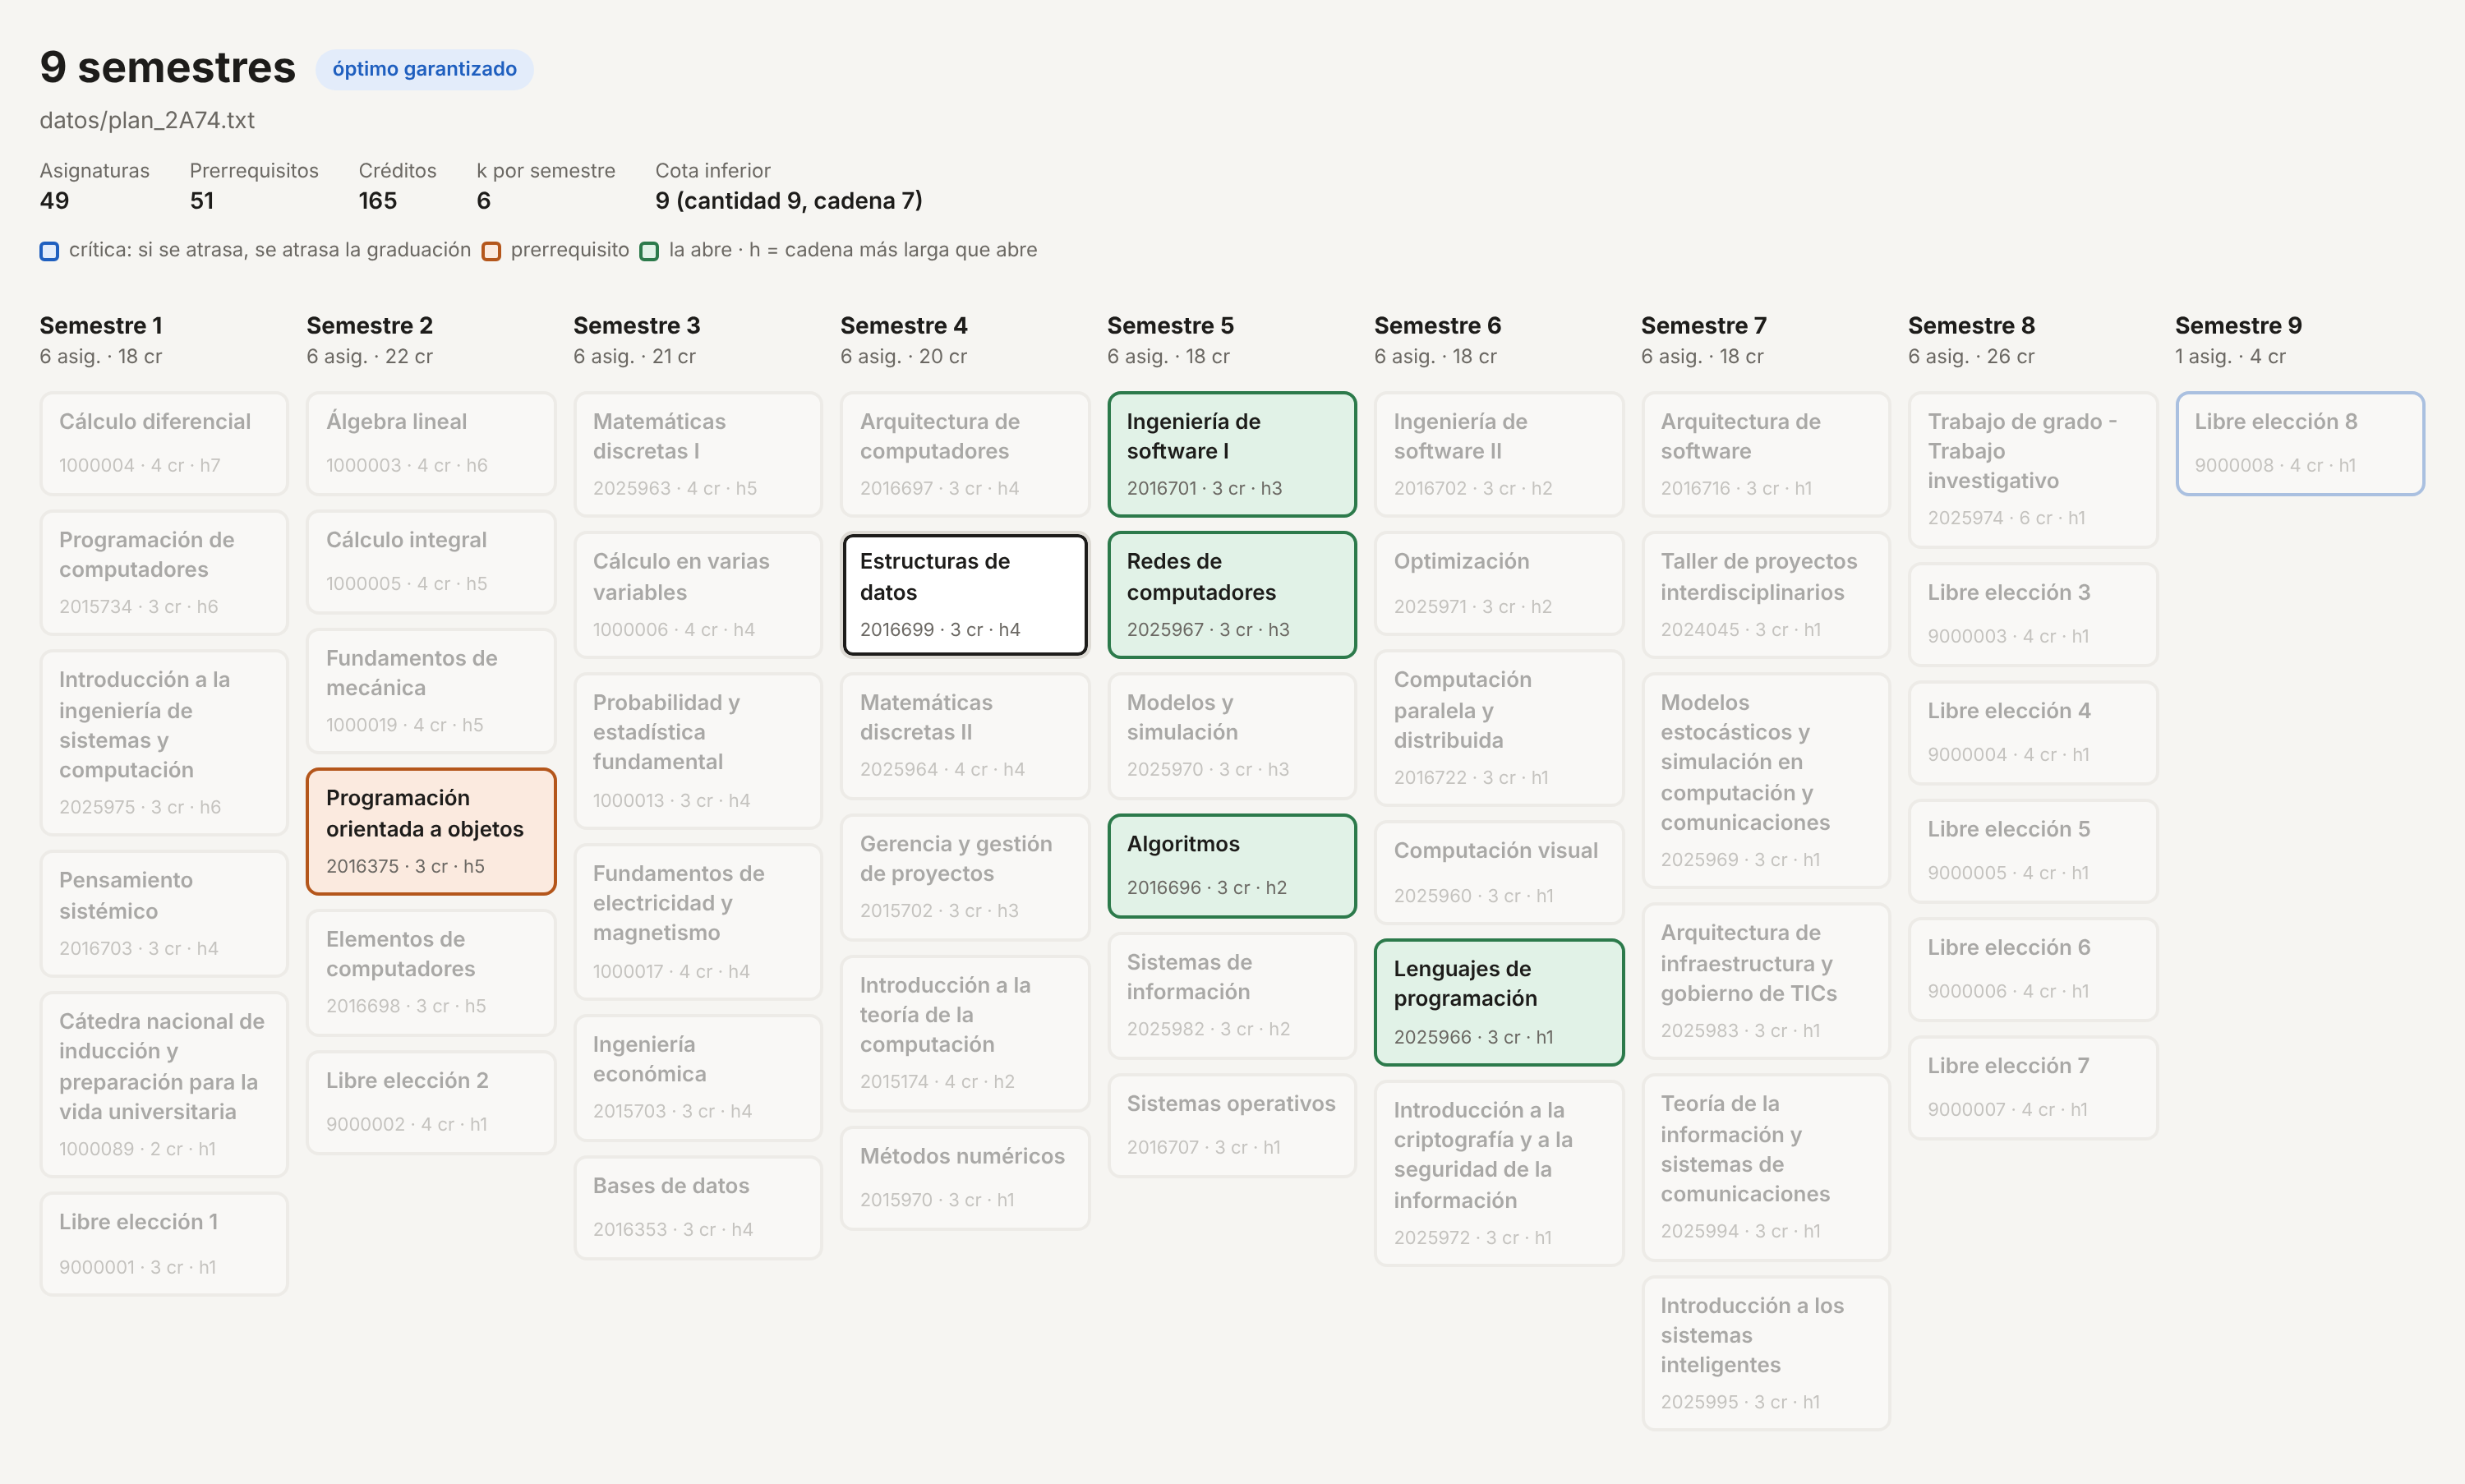
\includegraphics[width=\linewidth]{figuras/vista_html.png}
\caption{Vista HTML del plan de la malla con $k = 6$ (opción \texttt{--html}). Al pasar el puntero sobre Estructuras de datos se resaltan su prerrequisito (naranja) y las asignaturas que abre (verde); el borde azul marca las críticas.}
\label{fig:html}
\end{figure}

\subsection{Calidad de la cota en planes aleatorios}\label{sec:calidad}
\texttt{ExperimentoCalidad} genera 300 planes por cada combinación de familia, $n \in \{20, 50, 100, 200\}$ y $k \in \{2, \dots, 6\}$: \num{12000} planes en total. La familia \emph{general} tiene hasta 3 prerrequisitos por asignatura, elegidos entre cualquier asignatura anterior; en la familia \emph{árbol de ensamble} cada asignatura es prerrequisito de a lo sumo otra. Las semillas son fijas, así que los resultados son los mismos en cualquier computador. Se ejecuta con \texttt{--calidad}.

\begin{table}[H]
\centering
\small
\caption{Porcentaje de planes certificados como óptimos (promedio de $k = 2$ a $6$; 1500 planes por fila).}
\label{tab:calidad}
\begin{tabular}{@{}l r r r r@{}}
\toprule
\textbf{Familia} & $n$ & \textbf{Cota simple} & \textbf{Cota reforzada} & \textbf{Brecha máxima} \\
\midrule
General & 20 & 97,8 \% & 97,8 \% & 1 \\
 & 50 & 99,0 \% & 99,0 \% & 2 \\
 & 100 & 100,0 \% & 100,0 \% & 0 \\
 & 200 & 100,0 \% & 100,0 \% & 0 \\
\addlinespace
Árbol de ensamble & 20 & 97,5 \% & 100,0 \% & 0 \\
 & 50 & 94,1 \% & 100,0 \% & 0 \\
 & 100 & 89,1 \% & 100,0 \% & 0 \\
 & 200 & 86,7 \% & 100,0 \% & 0 \\
\midrule
General, total & & 99,2 \% & 99,2 \% & 2 \\
Árbol, total & & 91,9 \% & 100,0 \% & 0 \\
\bottomrule
\end{tabular}
\end{table}

En los árboles de ensamble el algoritmo de Hu es óptimo, y la cota reforzada lo certifica en todos los casos, mientras que la simple falla en el 8,1~\% (figura~\ref{fig:calidad}). En la familia general, los 48 planes no certificados tienen una brecha de 1 semestre, salvo uno con brecha de 2; el resultado de esos planes puede ser óptimo de todos modos.

\begin{figure}[H]
\centering
\begin{tikzpicture}
\begin{axis}[
  estilo,
  width=0.56\linewidth, height=6.2cm,
  xlabel={$k$ (máximo de asignaturas por semestre)},
  ylabel={Planes certificados (\%)},
  xtick={2,3,4,5,6}, ymin=72, ymax=102,
  legend style={at={(1.04,0.5)}, anchor=west},
]
\addplot coordinates {(2,91.333) (3,97.333) (4,99.333) (5,99.667) (6,100)};
\addlegendentry{Cota simple, $n = 20$}
\addplot coordinates {(2,81.667) (3,93.0) (4,96.667) (5,99.333) (6,100)};
\addlegendentry{Cota simple, $n = 50$}
\addplot coordinates {(2,76.333) (3,81.667) (4,92.667) (5,96.333) (6,98.333)};
\addlegendentry{Cota simple, $n = 100$}
\addplot coordinates {(2,80.667) (3,80.667) (4,84.0) (5,91.667) (6,96.333)};
\addlegendentry{Cota simple, $n = 200$}
\addplot[black, very thick, dashed, mark=none] coordinates {(2,100) (6,100)};
\addlegendentry{Cota reforzada (todos los $n$)}
\end{axis}
\end{tikzpicture}
\caption{Árboles de ensamble: porcentaje de planes que cada cota certifica como óptimos, por $k$ y $n$.}
\label{fig:calidad}
\end{figure}

% =============================================================================
\needspace{8\baselineskip}
\section{Análisis de rendimiento y complejidad}\label{sec:rendimiento}

\subsection{Metodología}
\begin{itemize}
\item \textbf{Herramientas}: Java (código de nivel 17, ejecutado con OpenJDK 24.0.2) y el cronómetro \texttt{System.nanoTime()}, que es monótono y tiene resolución de nanosegundos~\cite{oracle2021}. No se usaron librerías de medición, para mantener el proyecto sin dependencias.
\item \textbf{Datos}: planes aleatorios de \texttt{GeneradorPlanes}, acíclicos por construcción (cada asignatura toma prerrequisitos solo entre las generadas antes), con hasta 3 prerrequisitos elegidos entre las 100 anteriores ($e \approx 1{,}5\,n$), IDs dispersos y barajados con Fisher--Yates, y $k = 5$. El generador es SplitMix64~\cite{steele2014}, implementado en el proyecto.
\item \textbf{Tamaños}: $n = 10^4$, $2 \cdot 10^4$, $5 \cdot 10^4$, $10^5$, $2 \cdot 10^5$, $5 \cdot 10^5$ y $10^6$.
\item \textbf{Repeticiones}: 5 por tamaño, cada una con otra semilla (2026, 2027, …); se reporta la mediana, que no se afecta por una corrida atípica.
\item \textbf{Calentamiento}: antes de medir se hacen 3 corridas con $n = 10^4$ que no se registran, porque el compilador JIT de Java optimiza el código durante las primeras ejecuciones.
\item \textbf{Aislamiento}: generar los datos, verificar el plan y llamar al recolector de basura quedan fuera de los tramos medidos, y nada se imprime dentro de ellos. Con $n \geq 10^5$ se llama al recolector antes de cada fase.
\item \textbf{Comparaciones $O(n^2)$}: la planificación con lista sin orden y la inserción de IDs ordenados en el BST solo se miden hasta $n = \num{20000}$. Para tener más puntos se corren aparte con $n$ de \num{1000} a \num{20000}.
\end{itemize}
Las mediciones se reproducen con:
\begin{lstlisting}[style=consola]
java -cp out unal.graduacion.Main --medir
java -cp out unal.graduacion.Main --medir --tamanos 1000,2000,5000,10000,20000 --csv resultados/cuadraticas.csv
\end{lstlisting}

Cada corrida escribe un CSV con una fila por repetición y un resumen con las medianas (\texttt{tiempos\_resumen.csv} y \texttt{cuadraticas\_resumen.csv}), que es lo que leen las tablas y gráficas de esta sección.

\subsection{Complejidad teórica}

\begin{table}[H]
\centering
\small
\caption{Complejidad de cada fase, con $n$ asignaturas, $e$ prerrequisitos, $H$ la cadena más larga, $T$ los semestres y $w$ las asignaturas que esperan créditos.}
\label{tab:complejidad}
\begin{tabularx}{\linewidth}{@{}l l L@{}}
\toprule
\textbf{Fase} & \textbf{Costo} & \textbf{Por qué} \\
\midrule
Registro & $O((n + e) \log n)$ & $n$ inserciones y $e$ búsquedas en el AVL por ID \\
Kahn & $O(n + e)$ & cada asignatura entra y sale de la cola una vez; cada arista se recorre una vez \\
Alturas & $O(n + e)$ & cada asignatura se desapila una vez; cada arista se recorre una vez \\
Planificación & $O(n \log n + e + T w)$ & cada asignatura entra y sale del AVL una vez; cada arista se descuenta una vez \\
Cota inferior & $O(n + H)$ & conteo por altura y un recorrido de las alturas \\
Verificación & $O(n + e)$ & cada asignatura y cada arista se revisan una vez \\
\midrule
Total & $O((n + e) \log n)$ & domina el AVL; memoria $O(n + e)$ \\
\bottomrule
\end{tabularx}
\end{table}

Si un tramo cuesta $O(n)$, el tiempo dividido entre $n$ debe mantenerse casi constante al crecer $n$, y si cuesta $O(n \log n)$, lo constante es el tiempo dividido entre $n \log_2 n$. En una gráfica log-log, una recta de pendiente 1 indica crecimiento lineal o casi lineal, y una de pendiente 2, cuadrático.

\subsection{Planes de la medición}
Los planes salen de semillas fijas (2026 más el número de la repetición). La altura del AVL por ID está siempre entre la mínima posible, $\lceil \log_2(n + 1) \rceil$, y la cota teórica del AVL, y en todas las corridas el plan alcanzó la cota inferior: en estos planes las cadenas son cortas frente a $n/k$, así que manda la cota por cantidad.

\begin{table}[H]
\centering
\small
\caption{Planes usados en la medición ($k = 5$; mediana de las 5 repeticiones).}
\label{tab:planes-medicion}
\begin{tabular}{@{}r r r r r r@{}}
\toprule
$n$ & $e$ & \textbf{Altura del AVL} & \textbf{Altura mínima} & \textbf{Cota del AVL} & \textbf{Semestres = cota} \\
\midrule
\num{10000} & \num{15132} & 16 & 14 & 18,8 & \num{2000} \\
\num{20000} & \num{30022} & 17 & 15 & 20,3 & \num{4000} \\
\num{50000} & \num{74829} & 19 & 16 & 22,2 & \num{10000} \\
\num{100000} & \num{150212} & 20 & 17 & 23,6 & \num{20000} \\
\num{200000} & \num{300323} & 21 & 18 & 25,0 & \num{40000} \\
\num{500000} & \num{749430} & 23 & 19 & 26,9 & \num{100000} \\
\num{1000000} & \num{1499738} & 24 & 20 & 28,4 & \num{200000} \\
\bottomrule
\end{tabular}
\end{table}

\subsection{Tiempos medidos}\label{sec:tiempos}
La tabla~\ref{tab:tiempos} muestra la mediana de cada fase en milisegundos, medida en el computador de la tabla~\ref{tab:equipo}, y la figura~\ref{fig:fases}, su crecimiento.

\begin{table}[H]
\centering
\small
\caption{Mediana del tiempo de cada fase (ms), con $k = 5$.}
\label{tab:tiempos}
\ifhaytiempos
\pgfplotstabletypeset[
  columns={n,registro_avl,validacion_kahn,alturas_pila,planificacion_avl,cota_inferior,proceso_total},
  every head row/.style={before row=\toprule, after row=\midrule},
  every last row/.style={after row=\bottomrule},
  columns/n/.style={column name={$n$}, int detect},
  columns/registro_avl/.style={column name={Registro}, fixed, fixed zerofill, precision=2},
  columns/validacion_kahn/.style={column name={Kahn}, fixed, fixed zerofill, precision=2},
  columns/alturas_pila/.style={column name={Alturas}, fixed, fixed zerofill, precision=2},
  columns/planificacion_avl/.style={column name={Planificación}, fixed, fixed zerofill, precision=2},
  columns/cota_inferior/.style={column name={Cota}, fixed, fixed zerofill, precision=3},
  columns/proceso_total/.style={column name={Total}, fixed, fixed zerofill, precision=2},
]{\tablaTiempos}
\else
\cajapendiente[2.6cm]{Tabla de tiempos. Se llena sola al compilar cuando \texttt{tiempos\_resumen.csv} está junto a este archivo (o en \texttt{../resultados/}).}
\fi
\end{table}

\begin{figure}[H]
\centering
\ifhaytiempos
\begin{tikzpicture}
\begin{loglogaxis}[
  estilo,
  width=0.85\linewidth, height=7.2cm,
  xlabel={$n$ (asignaturas)}, ylabel={Mediana (ms)},
  legend style={at={(0.5,-0.2)}, anchor=north, legend columns=3},
]
\addplot table[x=n, y=registro_avl] {\tablaTiempos};
\addlegendentry{Registro (AVL por ID)}
\addplot table[x=n, y=validacion_kahn] {\tablaTiempos};
\addlegendentry{Kahn (cola)}
\addplot table[x=n, y=alturas_pila] {\tablaTiempos};
\addlegendentry{Alturas (pila)}
\addplot table[x=n, y=planificacion_avl] {\tablaTiempos};
\addlegendentry{Planificación (AVL de prioridad)}
\addplot table[x=n, y=proceso_total] {\tablaTiempos};
\addlegendentry{Proceso total}
\end{loglogaxis}
\end{tikzpicture}
\else
\cajapendiente[5cm]{Gráfica log-log del tiempo de cada fase frente a $n$. Aparece sola con \texttt{tiempos\_resumen.csv}.}
\fi
\caption{Tiempo de cada fase frente al número de asignaturas, en escala log-log.}
\label{fig:fases}
\end{figure}

La figura~\ref{fig:normalizado} divide cada tiempo entre el crecimiento esperado. Si la teoría se cumple, las curvas deben ser casi horizontales.

\begin{figure}[H]
\centering
\ifhaytiempos
\begin{tikzpicture}
\begin{semilogxaxis}[
  estilo,
  width=0.5\linewidth, height=6.4cm,
  xlabel={$n$}, ylabel={ns por elemento ($t/n$)},
  title={\small Operaciones $O(n)$},
  ymin=0,
  legend style={at={(0.5,-0.24)}, anchor=north},
]
\addplot table[x=n, y expr={\thisrow{validacion_kahn}*1000000/\thisrow{n}}] {\tablaTiempos};
\addlegendentry{Kahn}
\addplot table[x=n, y expr={\thisrow{alturas_pila}*1000000/\thisrow{n}}] {\tablaTiempos};
\addlegendentry{Alturas}
\addplot table[x=n, y expr={\thisrow{lista_agregar_final}*1000000/\thisrow{n}}] {\tablaTiempos};
\addlegendentry{Lista: agregar}
\addplot table[x=n, y expr={\thisrow{cola_encolar_desencolar}*1000000/\thisrow{n}}] {\tablaTiempos};
\addlegendentry{Cola: encolar y desencolar}
\addplot table[x=n, y expr={\thisrow{pila_apilar_desapilar}*1000000/\thisrow{n}}] {\tablaTiempos};
\addlegendentry{Pila: apilar y desapilar}
\end{semilogxaxis}
\end{tikzpicture}%
\hfill
\begin{tikzpicture}
\begin{semilogxaxis}[
  estilo,
  width=0.5\linewidth, height=6.4cm,
  xlabel={$n$}, ylabel={ns por $n \log_2 n$},
  title={\small Operaciones $O(n \log n)$},
  ymin=0,
  legend style={at={(0.5,-0.24)}, anchor=north},
]
\addplot table[x=n, y expr={\thisrow{registro_avl}*1000000/(\thisrow{n}*ln(\thisrow{n})/ln(2))}] {\tablaTiempos};
\addlegendentry{Registro}
\addplot table[x=n, y expr={\thisrow{planificacion_avl}*1000000/(\thisrow{n}*ln(\thisrow{n})/ln(2))}] {\tablaTiempos};
\addlegendentry{Planificación}
\addplot table[x=n, y expr={\thisrow{avl_insertar}*1000000/(\thisrow{n}*ln(\thisrow{n})/ln(2))}] {\tablaTiempos};
\addlegendentry{AVL: insertar}
\addplot table[x=n, y expr={\thisrow{avl_buscar}*1000000/(\thisrow{n}*ln(\thisrow{n})/ln(2))}] {\tablaTiempos};
\addlegendentry{AVL: buscar}
\end{semilogxaxis}
\end{tikzpicture}
\else
\cajapendiente[5cm]{Dos gráficas: tiempo entre $n$ para las operaciones $O(n)$ y tiempo entre $n \log_2 n$ para las $O(n \log n)$. Aparecen solas con \texttt{tiempos\_resumen.csv}.}
\fi
\caption{Tiempos normalizados. Izquierda: nanosegundos por elemento de las operaciones lineales. Derecha: nanosegundos por $n \log_2 n$ de las operaciones con AVL.}
\label{fig:normalizado}
\end{figure}

\subsection{Comparación de estructuras}\label{sec:comparacion}
La tabla~\ref{tab:comparacion} y la figura~\ref{fig:comparacion} comparan el AVL con las dos alternativas: planificar con la lista sin orden e insertar IDs ordenados en un BST. Las alturas no dependen del computador: con IDs ordenados, el BST queda con altura $n$ y el AVL con la mínima posible, $\lceil \log_2(n + 1) \rceil$ (15 con $n = \num{20000}$).

\begin{table}[H]
\centering
\small
\caption{AVL frente a las alternativas $O(n^2)$ (mediana en ms).}
\label{tab:comparacion}
\ifhaycuadraticas
\pgfplotstabletypeset[
  columns={n,planificacion_avl,planificacion_lista,razon_lista,avl_insertar_ordenados,bst_insertar_ordenados,razon_bst,altura_avl_ordenados,altura_bst_ordenados},
  every head row/.style={
    before row={\toprule & \multicolumn{3}{c}{Planificación} & \multicolumn{3}{c}{Insertar IDs ordenados} & \multicolumn{2}{c}{Altura}\\
      \cmidrule(lr){2-4}\cmidrule(lr){5-7}\cmidrule(l){8-9}},
    after row=\midrule},
  every last row/.style={after row=\bottomrule},
  columns/n/.style={column name={$n$}, int detect},
  columns/planificacion_avl/.style={column name={AVL}, fixed, fixed zerofill, precision=2},
  columns/planificacion_lista/.style={column name={Lista}, fixed, fixed zerofill, precision=1},
  columns/razon_lista/.style={column name={Lista/AVL}, fixed, precision=0, postproc cell content/.append style={/pgfplots/table/@cell content/.add={}{$\times$}}},
  columns/avl_insertar_ordenados/.style={column name={AVL}, fixed, fixed zerofill, precision=2},
  columns/bst_insertar_ordenados/.style={column name={BST}, fixed, fixed zerofill, precision=1},
  columns/razon_bst/.style={column name={BST/AVL}, fixed, precision=0, postproc cell content/.append style={/pgfplots/table/@cell content/.add={}{$\times$}}},
  columns/altura_avl_ordenados/.style={column name={AVL}, int detect},
  columns/altura_bst_ordenados/.style={column name={BST}, int detect},
]{\tablaCuadraticas}
\else
\cajapendiente[2.6cm]{Tabla de la comparación. Se llena sola con \texttt{cuadraticas\_resumen.csv} (segunda corrida de la metodología).}
\fi
\end{table}

\begin{figure}[H]
\centering
\ifhaycuadraticas
\begin{tikzpicture}
\begin{loglogaxis}[
  estilo,
  width=0.85\linewidth, height=7cm,
  xlabel={$n$ (asignaturas)}, ylabel={Mediana (ms)},
  legend style={at={(0.5,-0.2)}, anchor=north, legend columns=2},
]
\addplot table[x=n, y=planificacion_lista] {\tablaCuadraticas};
\addlegendentry{Planificación con lista sin orden}
\addplot table[x=n, y=planificacion_avl] {\tablaCuadraticas};
\addlegendentry{Planificación con AVL}
\addplot table[x=n, y=bst_insertar_ordenados] {\tablaCuadraticas};
\addlegendentry{BST con IDs ordenados}
\addplot table[x=n, y=avl_insertar_ordenados] {\tablaCuadraticas};
\addlegendentry{AVL con IDs ordenados}
\end{loglogaxis}
\end{tikzpicture}
\else
\cajapendiente[5cm]{Gráfica log-log de la comparación. Aparece sola con \texttt{cuadraticas\_resumen.csv}.}
\fi
\caption{AVL frente a las alternativas. En escala log-log, las alternativas crecen con pendiente cercana a 2 y el AVL, cercana a 1.}
\label{fig:comparacion}
\end{figure}

\subsection{Comparación entre la teoría y lo medido}
\paragraph{Crecimiento de las fases.} Entre $10^4$ y $10^6$ asignaturas, la pendiente de cada curva de la figura~\ref{fig:fases} es 1,16 para Kahn, 1,13 para las alturas, 1,13 para la planificación, 1,36 para el registro y 1,24 para el proceso total. Una fase $O(n)$ tendría pendiente 1 y una $O(n \log n)$, cerca de 1,09 en este rango, así que la planificación y las fases lineales quedan muy cerca de la teoría. El proceso completo, con un millón de asignaturas y 1,5 millones de prerrequisitos, tarda 4,9~s.

\paragraph{Tiempos normalizados.} En la figura~\ref{fig:normalizado}, la cola se mantiene entre 19 y 30~ns por elemento y la pila entre 6 y 18~ns, como corresponde a operaciones $O(1)$. La planificación se mantiene entre 42 y 74~ns por $n \log_2 n$. Kahn y las alturas se mantienen casi constantes hasta $5 \cdot 10^5$ asignaturas (entre 225 y 330~ns, y entre 62 y 122~ns por asignatura) y suben con $10^6$.

\paragraph{Lo que se sale de la tendencia.} El registro en el AVL por ID pasa de 40 a 142~ns por $n \log_2 n$, y casi todo ese aumento ocurre entre $10^4$ y $10^5$. Como los IDs llegan desordenados, cada búsqueda recorre nodos dispersos en la memoria; mientras el árbol cabe en la memoria caché del procesador esos accesos son rápidos, y cuando deja de caber cada visita espera a la RAM. El análisis $O(\cdot)$ supone que todos los accesos cuestan lo mismo, y esa diferencia explica que la pendiente sea mayor que la teórica; de $10^5$ a $10^6$ el valor solo crece 1,3 veces. Insertar y buscar en el AVL muestran lo mismo en menor medida. Agregar al final de la lista pasa de 5--8~ns a 69--131~ns por elemento desde $10^5$: cada nodo es un objeto nuevo, y con cientos de miles de nodos el recolector de basura de Java tiene que copiarlos, un costo que el análisis teórico no incluye. Por los mismos efectos, al multiplicar $n$ por 10 el proceso total crece 19,8 veces de $10^4$ a $10^5$ y 15,5 veces de $10^5$ a $10^6$, algo más que las 12 veces que predice $O(n \log n)$.

\paragraph{Comparación con las alternativas.} Con $n = \num{20000}$, planificar con la lista sin orden es 60 veces más lento que con el AVL (855,6 frente a 14,3~ms), e insertar los IDs ordenados en el BST es 191 veces más lento que en el AVL (483,8 frente a 2,5~ms), como muestra la tabla~\ref{tab:comparacion}. Entre \num{1000} y \num{20000} asignaturas, la lista crece con pendiente 2,08 y el BST con 1,90, como corresponde a $O(n^2)$, mientras que el AVL crece con 1,05 en la planificación y 0,93 en la inserción ordenada. Al duplicar $n$ de \num{10000} a \num{20000}, el BST tarda 4,0 veces más, justo lo que predice $O(n^2)$, y el AVL 2,3 veces. La ventaja del AVL crece con $n$: con \num{1000} asignaturas la lista es 3 veces más lenta, y con \num{20000}, 60 veces.

\subsection{Dificultades y ajustes}
\begin{itemize}
\item \textbf{Calentamiento de la JVM}: las primeras corridas eran más lentas por el compilador JIT; se agregaron 3 corridas de calentamiento que no se registran.
\item \textbf{Recolector de basura}: con planes grandes podía activarse dentro de un tramo medido; se llama antes de cada fase y se reporta la mediana.
\item \textbf{Caso degenerado del BST}: con \num{20000} IDs ordenados, una inserción recursiva desbordaría la pila de llamadas de Java; el BST se implementó de forma iterativa.
\item \textbf{Alternativas cuadráticas}: pasar de $2 \cdot 10^4$ a $10^6$ asignaturas multiplicaría su tiempo por \num{2500}, así que solo se miden hasta \num{20000}.
\item \textbf{Formato de los CSV}: con la configuración regional en español, Java escribe los decimales con coma, y eso rompe el formato CSV; los números se escriben con punto sin depender de la configuración.
\item \textbf{JDK fuera del PATH}: en el computador de las mediciones \texttt{javac} no estaba en el PATH, y el JDK instalado aparte era Java 8, más antiguo que el que necesita el proyecto. El script de mediciones busca un JDK 17 o superior en las carpetas de instalación habituales y usó el que trae Apache NetBeans.
\item \textbf{Variación entre corridas}: en un portátil la frecuencia del procesador cambia con la temperatura y la carga. En la corrida principal, insertar \num{20000} IDs ordenados en el BST tardó 897~ms, y en la corrida aparte, 484~ms. Por eso se reporta la mediana de 5 repeticiones; las conclusiones (pendiente cercana a 2 para las alternativas y cercana a 1 para el AVL) son las mismas en las dos corridas.
\item \textbf{Memoria}: con $n = 10^6$ bastó la memoria por defecto de la JVM (3,5~GB); no hizo falta la opción \texttt{-Xmx}.
\end{itemize}

% =============================================================================
\needspace{8\baselineskip}
\section{Conclusiones}\label{sec:conclusiones}
\begin{itemize}
\item El prototipo cumple los requisitos RF1 a RF7 con estructuras implementadas desde cero: registra las asignaturas con su ID y su lista de prerrequisitos en un AVL, accede a cualquiera por su ID, detecta ciclos, calcula los semestres y los muestra en consola y en HTML. Las 81 verificaciones funcionales pasan.
\item En la malla real del plan 2A74, el sistema encuentra un plan de 9 semestres con $k = 6$, uno menos que la malla sugerida, y demuestra con la cota inferior que no existe uno más corto. Lo mismo ocurre para todos los valores de $k$ probados.
\item Aunque el problema es NP-difícil en general, el algoritmo de Hu con la cota reforzada certificó el óptimo en el 99,2~\% de los planes aleatorios generales y en el 100~\% de los árboles de ensamble. La cota reforzada es necesaria: la simple deja sin certificar el 8,1~\% de los árboles.
\item Elegir un AVL en lugar de un BST evita el peor caso con IDs ordenados: con \num{20000} códigos, la altura pasa de \num{20000} a 15.
\item En un portátil con un procesador AMD Ryzen 3 3250U, el proceso completo con un millón de asignaturas tarda 4,9~s. Las fases crecen con pendientes de 1,13 a 1,36 en escala log-log, cerca de lo que predice la teoría; la diferencia se explica por la memoria caché y el recolector de basura.
\item Con \num{20000} asignaturas, la lista sin orden es 60 veces más lenta que el AVL y el BST con IDs ordenados, 191 veces, y la diferencia crece con $n$ porque esas alternativas son $O(n^2)$.
\end{itemize}

Para la Entrega 3 se reemplazará el AVL por ID por una tabla hash (acceso en $O(1)$ promedio), el AVL de prioridad por un heap de máximos (mismo $O(\log n)$ con menor costo constante, sobre un arreglo) y las listas sueltas por un grafo dirigido explícito. Además se agregará una solución exacta con conjuntos de bits para planes pequeños, para medir la brecha real en los casos que la cota no certifica.

% =============================================================================
\needspace{8\baselineskip}
\section{Video demostrativo}\label{sec:video}
Enlace: \pendiente{enlace al video (máximo 8 minutos)}

Contenido sugerido, en orden:
\begin{enumerate}
\item Clonar el repositorio desde GitHub, compilar y correr las pruebas (esta parte puede ir a velocidad x2).
\item Calcular el plan de la malla 2A74 con $k = 6$, consultar una asignatura por su código y cambiar $k$ desde el menú.
\item Mostrar un plan con ciclo y el archivo con errores.
\item Abrir la vista HTML del plan.
\item Explicar en el código las estructuras: AVL, cola, pila y listas.
\item Mostrar las mediciones, las gráficas de este reporte y la complejidad.
\item Justificar por qué la solución es la más adecuada y cerrar con las conclusiones.
\end{enumerate}

% =============================================================================
\begin{thebibliography}{99}
\addcontentsline{toc}{section}{Referencias}

\bibitem{avl1962} G.~M. Adelson-Velsky y E.~M. Landis, «An algorithm for the organization of information», \emph{Soviet Mathematics Doklady}, vol.~3, pp.~1259--1263, 1962.

\bibitem{brucker2007} P. Brucker, \emph{Scheduling Algorithms}, 5.ª ed. Berlín: Springer, 2007.

\bibitem{coffman1972} E.~G. Coffman y R.~L. Graham, «Optimal scheduling for two-processor systems», \emph{Acta Informatica}, vol.~1, n.º~3, pp.~200--213, 1972.

\bibitem{cormen2022} T.~H. Cormen, C.~E. Leiserson, R.~L. Rivest y C. Stein, \emph{Introduction to Algorithms}, 4.ª ed. Cambridge, MA: MIT Press, 2022.

\bibitem{garey1979} M.~R. Garey y D.~S. Johnson, \emph{Computers and Intractability: A Guide to the Theory of NP-Completeness}. Nueva York: W.~H. Freeman, 1979.

\bibitem{herrera2026} D.~A. Herrera Álvarez, «Proyecto de clase: Graduación UNAL. Enunciado y especificación de la Entrega 2», Estructuras de Datos (2016699), Universidad Nacional de Colombia, 2026.

\bibitem{hu1961} T.~C. Hu, «Parallel sequencing and assembly line problems», \emph{Operations Research}, vol.~9, n.º~6, pp.~841--848, 1961.

\bibitem{kahn1962} A.~B. Kahn, «Topological sorting of large networks», \emph{Communications of the ACM}, vol.~5, n.º~11, pp.~558--562, 1962.

\bibitem{knuth1998} D.~E. Knuth, \emph{The Art of Computer Programming, vol.~3: Sorting and Searching}, 2.ª ed. Reading, MA: Addison-Wesley, 1998.

\bibitem{lenstra1978} J.~K. Lenstra y A.~H.~G. Rinnooy Kan, «Complexity of scheduling under precedence constraints», \emph{Operations Research}, vol.~26, n.º~1, pp.~22--35, 1978.

\bibitem{oracle2021} Oracle, «Class System: nanoTime()», \emph{Java SE 17 \& JDK 17 API Specification}, 2021. [En línea]. Disponible en: \url{https://docs.oracle.com/en/java/javase/17/docs/api/java.base/java/lang/System.html}

\bibitem{steele2014} G.~L. Steele, D. Lea y C.~H. Flood, «Fast splittable pseudorandom number generators», en \emph{Proceedings of the 2014 ACM International Conference on Object Oriented Programming Systems Languages \& Applications (OOPSLA)}, pp.~453--472, 2014.

\bibitem{ullman1975} J.~D. Ullman, «NP-complete scheduling problems», \emph{Journal of Computer and System Sciences}, vol.~10, n.º~3, pp.~384--393, 1975.

\bibitem{acuerdo2023} Universidad Nacional de Colombia, Consejo de Facultad de Ingeniería, «Acuerdo 11 de 2023», Régimen Legal de la Universidad Nacional de Colombia, 2023. [En línea]. Disponible en: \url{https://legal.unal.edu.co/rlunal/home/doc.jsp?d_i=106142}

\bibitem{malla2023} Universidad Nacional de Colombia, Facultad de Ingeniería, «Malla curricular, plan de estudios estándar 2023: Ingeniería de Sistemas y Computación (2A74)», 2023.

\bibitem{weiss2012} M.~A. Weiss, \emph{Data Structures and Algorithm Analysis in Java}, 3.ª ed. Boston: Pearson, 2012.

\end{thebibliography}

\end{document}
